\chapter{高等数学}
	高等数学是硕士研究生招生考试考查内容之一,主要考查考生对高等数学的基本概念、基本理论、基本方法的理解和掌握以及考生的抽象思维能力、逻辑推理能力、综合运用能力和解决实际问题的能力。在考研数学一试卷中分值为82分,约占56\%。
		\section{极限、连续}
	\subsection{函数极限}
	\begin{ti}
		求 $\lim_{x\to 0} \frac{\sqrt{1+x} - 1 - \frac{x}{2}}{\ee^{x^{2}}-1}$.
	\end{ti}

	\begin{ti}
		求 $\lim_{x \to 0} \frac{\ee^{x} + \ln(1 - x) - 1}{x - \arctan x}$.
	\end{ti}

	\begin{ti}
		求 $\lim_{x \to 0} \frac{(1+x)^{\frac{2}{x}} - \ee^{2}[1 - \ln(1+x)]}{x}$.
	\end{ti}

	\begin{ti}
		求 $\lim_{x \to 0} \frac{\left(1 + x^{2}\right)(1 - \cos 2x) - 2x^{2}}{x^{4}}$.
	\end{ti}

	\begin{ti}
		求 $\lim_{x \to 0} \frac{\sqrt{1-x^{2}} \sin^{2}x - \tan^{2}x }{x^{2}[\ln(1+x)]^{2}}$.
	\end{ti}

	\begin{ti}
		求 $\lim_{x \to 0} \frac{(3 + 2 \tan x)^{x} - 3^{x}}{3 \sin^{2}x + x^{3} \cos\frac{1}{x}}$.
	\end{ti}

	\begin{ti}
		求 $\lim_{x \to 2}\frac{\sqrt{5x - 1} - \sqrt{2x + 5}}{x^{2} - 4}$.
	\end{ti}

	\begin{ti}
		求 $\lim_{x \to 0}\int_{0}^{x} \frac{\sin 2t}{\sqrt{4+t^{2}}\int_{0}^{x} \left(\sqrt{t+1} - 1\right)\dd{t}} \dd{t}$.
	\end{ti}

	\begin{ti}
		求 $\lim_{x \to \infty} \ee^{-x} \left( 1 + \frac{1}{x} \right)^{x^{2}}$.
	\end{ti}

	\begin{ti}
		求 $\lim_{x \to 3^{+}} \frac{\cos x \ln (x - 3)}{\ln\left( \ee^{x} - \ee^{3} \right)}$.
	\end{ti}

	\begin{ti}
		求 $\lim_{x \to \infty} x^{2} \left( a^{\frac{1}{x}} + a^{-\frac{1}{x}} - 2 \right)$,其中常数 $a > 0$.
	\end{ti}

	\begin{ti}
		求 $\lim_{x \to 0}\frac{1}{x}\left( \cot x - \frac{1}{x} \right)$.
	\end{ti}

	\begin{ti}
		求 $\lim_{x \to +\infty}\left( \sqrt[3]{x^{3} + 2x^{2} + 1} - x\ee^{\frac{1}{x}} \right)$.
	\end{ti}

	\begin{ti}
		求 $\lim_{x \to 0}\left( \frac{1+x}{1-e^{-x}} - \frac{1}{x} \right)$.
	\end{ti}

	\begin{ti}
		求 $\lim_{x \to 0^{+}} x^{\ln\left( \frac{\ln x - 1}{\ln x + 1} \right)}$.
	\end{ti}

	\begin{ti}
		求 $\lim_{x \to \infty} \left( \tan\frac{\uppi x}{1 + 2x} \right)^{\frac{1}{x}}$.
	\end{ti}

	\begin{ti}
		求 $\lim_{x \to 0^{+}} \left( \frac{\sin x}{x} \right)^{\frac{1}{1 - \cos x}}$.
	\end{ti}

	\begin{ti}
		求 $\lim_{x \to 0}\left( \frac{\cos x}{\cos 2x} \right)^{\frac{1}{x^{2}}}$.
	\end{ti}

	\begin{ti}
		求 $\lim_{x \to 0} \frac{\sin x - x\cos x}{x - \sin x}$.
	\end{ti}

	\begin{ti}
		求 $\lim_{x \to 0}\frac{1 + \frac{1}{2}x^{2} - \sqrt{1 + x^{2}}}{\left( \cos x - \ee^{\frac{x^{2}}{2}} \right) \sin \frac{x^{2}}{2}}$.
	\end{ti}

	\begin{ti}
		求 $\lim_{x \to \infty} \left( \sqrt[6]{x^{6} + x^{5}} - \sqrt[6]{x^{6} - x^{5}} \right)$.
	\end{ti}

	\begin{ti}
		求 $\lim_{x \to +\infty}\left[ \left( x^{3} + \frac{x}{2} - \tan \frac{1}{x} \right) \ee^{\frac{1}{x}} - \sqrt{1 + x^{6}} \right]$.
	\end{ti}

	\begin{ti}
		求 $\lim_{x \to 0}\frac{\ee^{\tan x} - \ee^{\sin x}}{x \sin^{2} x}$.
	\end{ti}

	\begin{ti}
		求 $\lim_{x \to 0} \frac{\sin x + x^{2} \sin\frac{1}{x}}{(1 + \cos x)\ln(1 + x)}$.
	\end{ti}

	\begin{ti}
		求 $\lim_{x \to 0}\left[ \frac{a}{x} - \left( \frac{1}{x^{2}} - a^{2} \right) \ln(1 + ax) \right]$,其中 $a \ne 0$.
	\end{ti}

	\begin{ti}
		求 $\lim_{x \to 0} \frac{(1 + x)^{\frac{1}{x}} - (1 + 2x)^{\frac{1}{2x}}}{\sin x}$.
	\end{ti}

	\begin{ti}
		求 $\lim_{x \to 0}\frac{\int_{0}^{\sin^{2}x} \ln(1 + t)\dd{t}}{\left( \sqrt[3]{1 + x^{3}} - 1 \right)\sin x}$.
	\end{ti}

	\begin{ti}
		求 $\lim_{x \to 0} \frac{ \int_{0}^{x} \left[ \int_{0}^{u^{2}} \arctan(1 + t) \dd{t} \right] \dd{u} }{x(1 - \cos x)}$.
	\end{ti}

	\begin{ti}
		求 $\lim_{x \to 0^{+}} \frac{x^{x} - ( \sin x )^{x}}{x^{2}\ln(1 + x)}$.
	\end{ti}

	\begin{ti}
		求 $\lim_{x \to 0} \frac{ \cos x - \ee^{-\frac{x^{2}}{2}} }{x^{2} [ x + \ln(1 - x) ]}$.
	\end{ti}

	\begin{ti}
		求 $\lim_{x \to 0} \frac{1}{x^{3}} \left[ \left( \frac{2 + \cos x}{3} \right)^{x} - 1 \right]$.
	\end{ti}

	\begin{ti}
		求 $\lim_{x \to 0} \frac{\ln\left( \sin^{2}x + \ee^{x} \right) - x}{\ln\left( x^{2} + \ee^{2x} \right) - 2x}$.
	\end{ti}

	\begin{ti}
		求 $\lim_{x \to 1} \frac{x - x^{x}}{1 - x + \ln x}$.
	\end{ti}

	\begin{ti}
		求 $\lim_{x \to 0} \left( \frac{a_{1}^{x} + a_{2}^{x} + \cdots + a_{n}^{x}}{n} \right)^{\frac{1}{x}}$,$a_{i} > 0$,且 $a_{i} \ne 1, i = 1,2,\cdots,n,n \geq 2$.
	\end{ti}

	\begin{ti}
		设 $\lim_{x \to 0} \frac{\ln\left[ 1 + \frac{f(x)}{\sin x} \right]}{a^{x} - 1} = A (a > 0, a \ne 1)$,求 $\lim_{x \to 0}\frac{f(x)}{x^{2}}$.
	\end{ti}

	\begin{ti}
		已知 $\lim_{x \to 1} f(x)$ 存在,且 $f(x) = \frac{x - \arctan(x - 1) - 1}{(x - 1)^{3}} + 2x^{2} \ee^{x-1} \cdot \lim_{x \to 1} f(x)$,求 $f(x)$.
	\end{ti}

	\begin{ti}
		设函数 $f(x) = (1 + x)^{\frac{1}{x}}(x > 0)$,证明:存在常数 $A,B$,使得当 $x \to 0^{+}$ 时,恒有
		\begin{equation*}
			f(x) = \ee + Ax +Bx^{2} + o\left( x^{2} \right),
		\end{equation*}
		并求常数 $A,B$.
	\end{ti}

	\begin{ti}
		已知 $\lim_{x \to 0} \frac{(1+x)^{\frac{1}{x}} - \left( A + Bx + Cx^{2} \right)}{x^{3}} = D \ne 0$. 求常数 $A,B,C,D$.
	\end{ti}

	\begin{ti}
		设函数 $f(x) = \begin{cases}
			\frac{\ln\left( 1 + x^{3} \right)}{\arcsin x - x}, & x < 0,\\
			\frac{\ee^{-x} + \frac{1}{2}x^{2} + x - 1}{x \sin \frac{x}{6}}, & x > 0,
		\end{cases}$,$g(x) = \frac{\ee^{\frac{1}{x}}\arctan\frac{1}{x}}{1 + \ee^{\frac{2}{x}}}$,求 $\lim_{x \to 0} f[g(x)]$.
	\end{ti}

	\begin{ti}
		设 $\alpha \geq 5$ 且为常数,则 $k$ 为何值时极限
		\begin{equation*}
			I = \lim_{x \to +\infty} \left[ \left( x^{\alpha} + 8x^{4} + 2 \right)^{k} - x \right]
		\end{equation*}
		存在,并求此极限值.
	\end{ti}
	
	\begin{ti}
		已知极限
		\[
			I = \lim_{x \to 0} \left( \frac{a}{x^{2}} + \frac{b}{x^{4}} + \frac{c}{x^{5}} \int_{0}^{x} \ee^{-t^{2}} \dd{t} \right) = 1,
		\]
		求常数 $a,b,c$.
	\end{ti}

	\begin{ti}
		求 $\lim_{x \to 0} \frac{ \sqrt{\cos x} - \sqrt[3]{\cos x} }{\sin^{2}x}$.
	\end{ti}

	\begin{ti}
		求 $\lim_{x \to 1} \frac{\left( 1 - \sqrt[3]{x} \right) \left( 1 - \sqrt[4]{x} \right) \cdots \left( 1 - \sqrt[n]{x} \right) }{(1 - x)^{n-2}}$.
	\end{ti}
	
	\begin{ti}
		求 $\lim_{x \to 0} \frac{1 - \cos x \cdot \sqrt{\cos 2x} \cdot \sqrt[3]{\cos 3x}}{x^{2}}$.
	\end{ti}

	\begin{ti}
		设函数 $f(x)$ 满足 $f(1) = 1$,且有 $f'(x) = \frac{1}{x^{2} + f^{2}(x)}$,证明:极限 $\lim_{x \to \infty} f(x)$ 存在,且极限值小于 $1 + \frac{\uppi}{4}$.
	\end{ti}

	\begin{ti}
		设 $x \geq 0$ 时,$f(x)$ 满足 $f'(x) = \frac{1}{x^{2} + f^{2}(x)}$,且 $f(0) = 1$,证明:$\lim_{x \to +\infty} f(x)$ 存在且极限值小于 $1 + \frac{\uppi}{2}$.
	\end{ti}
	\subsection{无穷小比阶}

	\begin{ti}
		当 $x \to 0$ ,$(1 - \cos x)\ln\left( 1 + 2x^{3} \right)$ 是比 $x \sin x^{n}$ 高阶的无穷小,而 $x \sin x^{n}$ 是比 $\ee^{x\tan^{2} x} - 1$ 高阶的无穷小,则正整数 $n = $ \htwo.
	\end{ti}

	\begin{ti}
		当 $x \to 0^{+}$ 时,$\sqrt{1 + \tan \sqrt{x}} - \sqrt{1 + \sin\sqrt{x}}$ 是 $x$ 的 $k$ 阶无穷小,则 $k =$ \htwo.
	\end{ti}

	\begin{ti}
		当 $x \to 0$ 时,$f(x) = \ln\left( 1+x^{2} \right) - 2\sqrt[3]{\left( \ee^{x} - 1 \right)^{2}}$ 是无穷小量 $x^{k}$ 的同阶无穷小,则 $k = $ \kuo.

		\fourch{$1$}{$2$}{$\frac{2}{3}$}{$\frac{3}{2}$}
	\end{ti}

	\begin{ti}
		当 $x \to 0$ 时,下列无穷小量中,最高阶的无穷小是\kuo.

		\twoch{$\ln\left( x + \sqrt{1 + x^{2}} \right)$}{$1 - \cos x$}{$\tan x - \sin x$}{$\ee^{x} + \ee^{-x} - 2$}
	\end{ti}

	\begin{ti}
		当 $x \to 0^{+}$ 时,下列无穷小量中,与 $x$ 同阶的无穷小是\kuo.

		\twoch{$\sqrt{1 + x} - 1$}{$\ln(1 + x) - x$}{$\cos(\sin x) - 1$}{$x^{x} - 1$}
	\end{ti}

	\begin{ti}
		当 $x \to 0$ 时,$f(x) = x - \sin x + \int_{0}^{x} t^{2} \ee^{t^{2}} \dd{t}$ 是 $x$ 的 $k$ 阶无穷小,则 $k=$ \kuo.

		\fourch{$3$}{$4$}{$5$}{$6$}
	\end{ti}

	\begin{ti}
		当 $x \to 0^{+}$ 时,试比较无穷小量 $\alpha$,$\beta$ 和 $\gamma$ 三者之间的阶,其中
		\[
			\alpha = \int_{0}^{x} \cos t^{2} \dd{t},\beta = \int_{0}^{x^{2}} \tan \sqrt{t} \dd{t},\gamma = \int_{0}^{\sqrt{x}} \sin t^{3} \dd{t}.
		\]
	\end{ti}

	\begin{ti}
		当 $x \to 0$ 时,$\sin x \left( \cos x - 4 \right) + 3x$ 为 $x$ 的几阶无穷小?
	\end{ti}

	\begin{ti}
		当 $x \to 0$ 时,确定下列无穷小量的阶数:
		\begin{enumerate}
			\item $\tan\left( \sqrt{x+2} - \sqrt{2} \right)$;
			\item $\sqrt[3]{1 + \sqrt[3]{x}} - 1$;
			\item $3^{\sqrt{x}} - 1$.  
		\end{enumerate}
	\end{ti}

	\begin{ti}
		当 $x \to 0$ 时,$x - \sin x \cos x \cos 2x$ 与 $cx^{k}$ 为等价无穷小,则 $c=$ \htwo,$k=$ \htwo.
	\end{ti}

	\begin{ti}
		当 $x \to 0$ 时,$1 - \cos x \cos 2x \cos 3x$ 对于无穷小 $x$ 的阶数等于 \htwo.
	\end{ti}

	\begin{ti}
		极限 $\lim_{x \to \infty} \frac{\ee^{\sin\frac{1}{x}}-1}{\left( 1 + \frac{1}{x} \right)^{\alpha} - \left( 1 + \frac{1}{x} \right)} = A \ne 0$ 的充要条件是 \kuo.

		\twoch{$\alpha > 1$}{$\alpha \ne 1$}{$\alpha > 0$}{与 $\alpha$ 无关}
	\end{ti}

	\begin{ti}
		设当 $x \to 0$ 时,$\ee^{\tan x} - \ee^{x}$ 与 $x^{n}$ 是同阶无穷小,则 $n$ 为 \kuo.

		\fourch{$1$}{$2$}{$3$}{$4$}
	\end{ti}

	\begin{ti}
		设当 $x \to 0$ 时,$f(x) = ax^{3} + bx$ 与 $g(x) =$ $\int_{0}^{\sin x} \left( \ee^{t^{2}} -1 \right) \dd{t}$ 是等价无穷小,则\kuo.

		\twoch{$a = \frac{1}{3},b=1$}{$a = 3,b=0$}{$a = \frac{1}{3},b=0$}{$a = 1,b=0$}
	\end{ti}

	\begin{ti}
		设当 $x \to 0$ 时,$f(x) = \ln\left( 1+x^{2} \right) - \ln\left( 1 + \sin^{2}x \right)$ 是 $x$ 的 $n$ 阶无穷小,则正整数 $n$ 为\kuo.
		
		\fourch{$1$}{$2$}{$3$}{$4$}
	\end{ti}

	\begin{ti}
		当 $x \to \uppi$ 时,若有 $\sqrt[4]{\sin\frac{x}{2}} - 1 \sim A(x - \uppi)^{k}$,则 $A=$\htwo,$k=$\htwo.
	\end{ti}

	\begin{ti}
		半径分别为 $R,r(R>r>0)$ 的两个圆相切于坐标轴原点. 如图~\ref{fig:1.1.1} 所示.
		\begin{enumerate}
			\item 当 $x \to 0^{+}$ 时,若线段长 $MM_{1}$ 与 $x^{k}$ 同阶,求 $k$;
			\item 当 $x \to 0^{+}$ 时,若 $\angle MOM_{1}$ 与 $x^{c}$ 同阶,求 $c$.
		\end{enumerate}
		\begin{figure}[htbp]
			\centering
			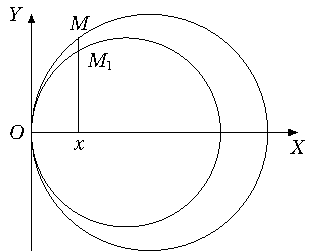
\includegraphics[scale=1]{figure/fig1-1-1.pdf}
			\caption{}\label{fig:1.1.1}
		\end{figure}
	\end{ti}
	\subsection{数列极限}

	\begin{ti}
		求 $\lim_{n \to \infty} n^{3} \left( \sin\frac{1}{n} - \frac{1}{2} \sin\frac{2}{n} \right)$.
	\end{ti}

	\begin{ti}
		求 $\lim_{n \to \infty} \left( \sqrt{n + 3\sqrt{n}} - \sqrt{n - \sqrt{n}} \right)$.
	\end{ti}

	\begin{ti}
		求 $\lim_{n \to \infty} \left[ \sqrt{n}\left( \sqrt{n+1} - \sqrt{n} \right) + \frac{1}{2} \right]^{\frac{\sqrt{n+1} + \sqrt{n}}{\sqrt{n+1} - \sqrt{n}}}$.
	\end{ti}

	\begin{ti}
		求 $\lim_{n \to \infty} n^{2} \left( a^{\frac{1}{n}} - a^{\frac{1}{n+1}} \right)$,其中 $a > 0$.
	\end{ti}

	\begin{ti}
		求 $\lim_{n \to \infty} \left( 1 + 2^{n} + 3^{n} \right)^{\frac{1}{n}}$.
	\end{ti}

	\begin{ti}
		求 $\lim_{n \to \infty} \cos\frac{x}{2}\cos\frac{x}{4}\cdots \cos\frac{x}{2^{n}}$.
	\end{ti}

	\begin{ti}
		求 $\lim_{n \to \infty} n^{2}\left( \arctan\frac{a}{n} - \arctan \frac{a}{n+1} \right)$,$a > 0$.
	\end{ti}

	\begin{ti}
		设 $\lim_{n \to \infty} \frac{n^{99}}{n^{k} - (n-1)^{k}}$ 存在且不为零,则常数 $k =$
		
		\noindent\hone{2}.
	\end{ti}

	\begin{ti}
		设数列 $\{ a_{n} \}$ 满足 $\lim_{n \to \infty}\frac{a_{n+1}}{a_{n}} = 1$,则\kuo.

		\twoch{$\{ a_{n} \}$ 有界}{$\{ a_{n} \}$ 不存在极限}{$\{ a_{n} \}$ 自某项起同号}{$\{ a_{n} \}$ 自某项起单调}
	\end{ti}

	\begin{ti}
		设数列 $\{ x_{n} \}$ 满足 $x_{n} > 0$,且 $\lim_{n \to \infty}\frac{x_{n+1}}{x_{n}} = \frac{1}{2}$,则\kuo.

		\onech{$\lim_{n\to\infty}x_{n} = 0$}{$\lim_{n\to\infty}x_{n}$ 存在,但不为零}{$\lim_{n\to\infty}x_{n}$ 不存在}{$\lim_{n\to\infty}x_{n}$ 可能存在,也可能不存在}
	\end{ti}

	\begin{ti}
		已知数列 $\{ a_{n} \}$ 单调,下列结论正确的是\kuo.
		
		\twoch{$\lim_{n \to \infty}\left( \ee^{a_{n}} - 1 \right)$ 存在}{$\lim_{n \to \infty} \frac{1}{1 + a_{n}^{2}}$ 存在}{$\lim_{n \to \infty} \sin a_{n}$ 存在}{$\lim_{n \to \infty} \frac{1}{1 - a_{n}^{2}}$ 存在}
	\end{ti}

	\begin{ti}
		设 $a_{1} = 1$,$a_{2} = 2$,$a_{n+2} = \frac{2a_{n}a_{n+1}}{a_{n} + a_{n+1}} (n=1,2,\cdots)$.
		\begin{enumerate}
			\item 求 $b_{n} = \frac{1}{a_{n+1}} - \frac{1}{a_{n}}$ 的表达式;
			\item 求 $\sum_{k=1}^{n} b_{k}$ 和 $\lim_{n \to \infty} a_{n}$.
		\end{enumerate}
	\end{ti}

	\begin{ti}
		设 $a_{1} = 3$,$a_{n+1} = a_{n}^{2} + a_{n}(n = 1,2,\cdots)$,求极限
		\[
			\lim_{n \to \infty} \left( \frac{1}{1 + a_{1}} + \frac{1}{1 + a_{2}} + \cdots + \frac{1}{1 + a_{n}} \right).
		\]
	\end{ti}
	
	\begin{ti}
		已知 $x_{1} = \frac{1}{2}$,$2 x_{n+1} + x_{n}^{2} = 1$,求 $\lim_{n \to \infty} x_{n}$.
	\end{ti}

	\begin{ti}
		设 $x_{1} = 1$,$x_{n} = 1 + \frac{1}{1 + x_{n-1}}(n = 2,3,\cdots)$. 证明 $\lim_{n \to \infty} x_{n}$ 存在,并求该极限.
	\end{ti}

	\begin{ti}
		设 $x_{1} = 1$,$x_{n+1} = \frac{x_{n} + 3}{x_{n} + 1}$,求 $\lim_{n \to \infty} x_{n}$.
	\end{ti}

	\begin{ti}
		设当 $a \leq x \leq b$ 时,$a \leq f(x) \leq b$,并设存在常数 $k$,$0 \leq k < 1$,对于 $[a,b]$ 上的任意两点 $x_{1}$ 与 $x_{2}$,都有 $|f(x_{1}) - f(x_{2})| \leq k |x_{1} - x_{2}|$. 证明:
		\begin{enumerate}
			\item 存在唯一的 $\xi \in [a,b]$ 使 $f(\xi) = \xi$;
			\item 对于任意给定的 $x_{1} \in [a,b]$,定义 $x_{n+1} = f(x_{n})$,$n = 1,2,\cdots$,则 $\lim_{n \to \infty} x_{n}$ 存在,且 $\lim_{n \to \infty} x_{n} = \xi$.
		\end{enumerate}
	\end{ti}

	\begin{ti}
		已知 $\left( 2 + \sqrt{2} \right)^{n} = A_{n} + B_{n}\sqrt{2}$,$A_{n},B_{n}$ 为整数,$n = 1,2,3,\cdots$,求 $\lim_{n\to \infty} \frac{A_{n}}{B_{n}}$.
	\end{ti}

	\begin{ti}
		设 $f(x)$ 在 $[0,+\infty)$ 上连续,满足 $0 \leq f(x) \leq x, x \in [0,+\infty)$,设 $a_{1} \geq 0$,$a_{n+1} = f(a_{n})(n = 1,2,\cdots)$,证明:
		\begin{enumerate}
			\item $\{ a_{n} \}$ 为收敛数列;
			\item 设 $\lim_{n \to \infty} a_{n} = t$,则有 $f(t) = t$;
			\item 若条件改为 $0 \leq f(x) < x,x \in (0,+\infty)$,则 $t = 0$.
		\end{enumerate}
	\end{ti}

	\begin{ti}
		\begin{enumerate}
			\item 设 $f(x) = x + \ln(2 - x)$,求 $f(x)$ 的最大值;
			\item 设 $x_{1} = \ln 2$,$x_{n} = \sum_{i=1}^{n-1} \ln(2 - x_{i}), n = 2,3,\cdots$,证明 $\lim_{n \to \infty} x_{n}$ 存在并求其极限值.
		\end{enumerate}
	\end{ti}

	\begin{ti}
		设 $x_{1} = 1$,$x_{n} = \int_{0}^{1} \min\{x,x_{n-1}\} \dd{x}, n = 2,3,\cdots$,证明 $\lim_{n \to \infty} x_{n}$ 存在并求其极限值.
	\end{ti}

	\begin{ti}
		设数列 $\{ x_{n} \}$ 满足 $0 < x_{1} < 1$,$\ln(1 + x_{n}) = \ee^{x_{n+1}} - 1(n = 1,2,\cdots)$,证明
		\begin{enumerate}
			\item 当 $0 < x < 1$ 时,$\ln(1 + x) < x < \ee^{x} - 1$;
			\item $\lim_{n \to \infty} x_{n}$ 存在,并求该极限.
		\end{enumerate}
	\end{ti}

	\begin{ti}
		\begin{enumerate}
			\item 证明方程 $x = 2\ln(1 + x)$ 在 $(0,+\infty)$ 内有唯一实根 $\xi$;
			\item 任取 $x_{1} > \xi$,定义 $x_{n+1} = 2\ln(1 + x_{n}), n = 1,2,\cdots$,证明 $\lim_{n \to \infty} x_{n} = \xi$.
		\end{enumerate}
	\end{ti}

	\begin{ti}
		\begin{enumerate}
			\item 证明方程 $\ee^{x} + x^{2n+1} = 0$ 在 $(-1,0)$ 内有唯一实根 $x_{n}, n = 0,1,2,\cdots$;
			\item 证明 $\lim_{n \to \infty} x_{n}$ 存在并求其值 $a$;
			\item 求 $\lim_{n \to \infty} n(x_{n} - a)$.
		\end{enumerate}
	\end{ti}

	\begin{ti}
		设 $F(x,y) = \frac{f(y - x)}{2x}$,$F(1,y) = \frac{y^{2}}{2} - y + 5$,$x_{0} > 0$,$x_{1} = F(x_{0},2x_{0})$,$\cdots$,$x_{n+1} = F(x_{n},2x_{n}), n = 1,2,\cdots$. 证明 $\lim_{n \to \infty} x_{n}$ 存在,并求该极限.
	\end{ti}

	\begin{ti}
		已知
		\[
			f_{n}(x) = \CC_{n}^{1} \cos x - \CC_{n}^{2} \cos^{2}x + \cdots + (-1)^{n-1} \CC_{n}^{n} \cos^{n}x.
		\]
		\begin{enumerate}
			\item 证明方程 $f_{n}(x) = \frac{1}{2}$ 在区间 $\left( 0,\frac{\uppi}{2} \right)$ 中仅有一根 $x_{n}, n = 1,2,3,\cdots$;
			\item 求 $\lim_{n \to \infty} f_{n}\left( \arccos\frac{1}{n} \right)$;
			\item 设 $x_{n} \in \left( 0,\frac{\uppi}{2} \right)$ 满足 $f_{n}(x_{n}) = \frac{1}{2}$,证明 $\lim_{n \to \infty} x_{n} = \frac{\uppi}{2}$.
		\end{enumerate}
	\end{ti}

	\begin{ti}
		\begin{enumerate}
			\item 证明:当 $x \to 0^{+}$ 时,不等式 $0 < \tan^{2}x - x^{2} < x^{4}$ 成立;
			\item 设 $x_{n} = \sum_{k=1}^{n} \tan^{2}\frac{1}{\sqrt{n+k}}$,求 $\lim_{n \to \infty}x_{n}$.
		\end{enumerate}
	\end{ti}

	\begin{ti}
		\begin{enumerate}
			\item 设 $f(x)$ 在 $(0,+\infty)$ 内可导,$f'(x) > 0, x \in (0,+\infty)$,证明 $f(x)$ 在 $(0,+\infty)$ 内单调增加;
			\item 证明 $f(x) = \left( n^{x} + 1 \right)^{-\frac{1}{x}}$ 在 $(0,+\infty)$ 内单调增加,其中 $n$ 为正整数;
			\item 设数列 $x_{n} = \sum_{k=1}^{n} \left( n^{k} + 1 \right)^{-\frac{1}{k}}$,求 $\lim_{n \to \infty} x_{n}$.
		\end{enumerate}
	\end{ti}
	\subsection{连续与间断}

	\begin{ti}
		当 $x \in \left( -\frac{1}{2},1 \right]$ 时,确定函数 $f(x) = \frac{\tan \uppi x}{|x|\left( x^{2} - 1 \right)}$ 的间断点,并判定其类型.
	\end{ti}

	\begin{ti}
		确定函数 $f(x) = \frac{x(x - 1)}{|x| x^{2} - |x|}$ 的间断点,并判定其类型.
	\end{ti}

	\begin{ti}
		设 $a > 0$,$b > 0$,$c > 0$,
		\[
			A(x) = \begin{cases}
				\left( \frac{a^{x} + b^{x}}{2} \right)^{\frac{1}{x}}, & x \ne 0,\\
				c, & x = 0.
			\end{cases}
		\]
		\begin{enumerate}
			\item 讨论 $A(x)$ 在 $x = 0$ 处的连续性;
			\item 讨论 $\lim_{x \to +\infty} A(x)$,$\lim_{x \to -\infty} A(x)$,$\lim_{x \to 0} A(x)$,$A(-1)$,$A(1)$ 五者之间的大小关系.
		\end{enumerate}
	\end{ti}

	\begin{ti}
		求 $f(x) = \frac{1}{1 - \ee^{\frac{x}{1 - x}}}$ 的连续区间、间断点,并判别间断点的类型.
	\end{ti}

	\begin{ti}
		求函数 $f(x) = \lim_{n \to \infty} \frac{x^{n+2} - x^{-n}}{x^{n} + x^{-n}}$ 的间断点并指出其类型.
	\end{ti}

	\begin{ti}
		若
		\[
			f(x) = \frac{\sqrt[3]{x}}{\lambda - \ee^{-kx}}
		\]
		在 $(-\infty,+\infty)$ 内连续,且 $\lim_{x \to -\infty} f(x) = 0$,则\kuo.
		
		\twoch{$\lambda < 0, k < 0$}{$\lambda < 0, k > 0$}{$\lambda \geq 0, k < 0$}{$\lambda \leq 0, k > 0$}
	\end{ti}

	\begin{ti}
		若
		\[
			f(x) = \begin{cases}
				\ee^{x} (\sin x + \cos x), & x > 0,\\
				2x + a, & x \leq 0
			\end{cases}
		\]
		 是 $(-\infty,+\infty)$ 内的连续函数,则 $a =$\hone{2}.
	\end{ti}

	\begin{ti}
		试讨论函数 $g(x) = \begin{cases}
			x^{\alpha} \sin\frac{1}{x}, & x > 0,\\
			\ee^{x} + \beta, & x \leq 0
		\end{cases}$ 在点 $x = 0$ 处的连续性.
	\end{ti}

	\begin{ti}
		求函数 $F(x) = \begin{cases}
			\frac{x(\uppi + 2x)}{2 \cos x}, & x \leq 0,\\
			\sin\frac{1}{x^{2} - 1}, & x > 0
		\end{cases}$ 的间断点,并判断它们的类型.
	\end{ti}

	\begin{ti}
		设 $f(x) = \lim_{n \to \infty}\frac{\ee^{\frac{1}{x}} \arctan\frac{1}{1 + x}}{x^{2} + \ee^{nx}}$,求 $f(x)$ 的间断点并判定其类型.
	\end{ti}

	\begin{ti}
		设 $f(x) = \begin{cases}
			\ee^{\frac{1}{x - 1}}, & x > 0,\\
			\ln(1 + x), & -1 < x < 0,
		\end{cases}$ 求 $f(x)$ 的间断点,并说明间断点的类型.
	\end{ti}

	\begin{ti}
		设 $f(x;t) = \left( \frac{x - 1}{t - 1} \right)^{\frac{t}{x - t}}((x - 1)(t - 1)>0, x \ne t)$,函数 $f(x)$ 由表达式
		\[
			f(x) = \lim_{t \to x}f(x;t)
		\]
		确定,求 $f(x)$ 的连续区间和间断点,并判定间断点的类型.
	\end{ti}

	\begin{ti}
		设函数 $f(x)$ 在 $[a,b]$ 上连续,$x_{1},x_{2},\cdots,x_{n},\cdots$ 是 $[a,b]$ 上的一个点列,求 $\lim_{n \to \infty} \sqrt[n]{\frac{1}{n}\sum_{k=1}^{n}\ee^{f(x_{k})}}$.
	\end{ti}

	\begin{ti}
		\begin{enumerate}
			\item 求函数 $f(x) = \lim_{n \to \infty} \sqrt[n]{1 + (2x)^{n} + x^{2n}}(x \geq 0)$ 的表达式;
			\item 讨论函数 $f(x)$ 的连续性.
		\end{enumerate}
	\end{ti}

	\begin{ti}
		已知 $f(x) = \lim_{n \to \infty} \frac{x^{2n-1} + ax^{2} + bx}{x^{2n} + 1}$ 是连续函数,求 $a,b$ 的值.
	\end{ti}

	\begin{ti}
		求函数 $f(x) = \frac{x^{3} + 1}{|x + 1|\left( x^{2} - x \right)} \sin\left( \frac{|x - 1|}{x + 2}\uppi \right)$ 的所有间断点,并判断它们的类型.
	\end{ti}
	\section{一元函数微分学}
	\subsection{一点的导数问题}

	\begin{ti}
		设 $f(x)$ 在 $x = 1$ 处可导,$f'(1) = 1$,求 $\lim_{x \to 1} \frac{f(x) - f(1)}{x^{10} - 1}$.
	\end{ti}

	\begin{ti}
		设 $f(x)$ 在 $x = 0$ 处连续,且 $\lim_{x \to 0} \left[ \frac{\ee^{f(x)} - \cos x + \sin x}{x} \right] = 0$,求 $f(0)$,并讨论 $f(x)$ 在 $x = 0$ 处是否可导?若可导,请求出 $f'(0)$.
	\end{ti}

	\begin{ti}
		函数 $f(x)$ 在 $(-\infty,+\infty)$ 内有定义,在区间 $[0,2]$ 上,$f(x) = x\left( x^{2} - 4 \right)$. 假若对任意的 $x$ 都满足 $f(x) = k f(x + 2)$,其中 $k$ 为常数.
		\begin{enumerate}
			\item 写出 $f(x)$ 在 $[-2,0)$ 上的表达式;
			\item 问 $k$ 为何值时,$f(x)$ 在 $x = 0$ 处可导?
		\end{enumerate}
	\end{ti}

	\begin{ti}
		设 $f(x)$ 在 $(-\infty,+\infty)$ 内有定义,且 $f'(0) = a(a \ne 0)$,又对任意的 $x,y \in (-\infty,+\infty)$,有
		\[
			f(x + y) = \frac{f(x) + f(y)}{1 - f(x)f(y)},
		\]
		求 $f(x)$.
	\end{ti}
	
	\begin{ti}
		设 $f(x)$ 在 $(-\infty,+\infty)$ 内有定义,且对任意的 $x,x_{1},x_{2} \in (-\infty,+\infty)$,有
		\[
			f(x_{1} + x_{2}) = f(x_{1}) \cdot f(x_{2}),f(x) = 1 + xg(x),
		\]
		其中 $\lim_{x \to 0} g(x) = 1$. 证明:$f(x)$ 在 $(-\infty,+\infty)$ 内处处可导.
	\end{ti}

	\begin{ti}
		设 $f(x)$ 定义在 $\mathbb{R}$ 上,对于任意的 $x_{1},x_{2}$,有 $|f(x_{1}) - f(x_{2})| \leq (x_{1} - x_{2})^{2}$,求证:$f(x)$ 是常值函数.
	\end{ti}

	\begin{ti}
		设 $f''(1)$ 存在,且 $\lim_{x \to 1}\frac{f(x)}{x - 1} = 0$. 记
		\[
			\varphi(x) = \int_{0}^{1} f'[1 + (x - 1)t]\dd{t}.
		\]
		求 $\varphi(x)$ 在 $x = 1$ 的某个邻域内的导数,并讨论 $\varphi'(x)$ 在 $x = 1$ 处的连续性.
	\end{ti}

	\begin{ti}
		设函数
		\[
			f(x) = \begin{cases}
				x^{3} \sin\frac{1}{x}, & x \ne 0,\\
				0, & x = 0.
			\end{cases}
		\]
		讨论 $f(x)$ 在 $x = 0$ 的可导性以及 $f'(x)$ 在 $x = 0$ 的连续性.
	\end{ti}

	\begin{ti}
		已知函数 $f(x) = \begin{cases}
			\frac{\int_{x}^{2x} \ee^{t^{2}} \dd{t}}{x}, & x \ne 0,\\
			a, & x = 0
		\end{cases}$ 在 $x = 0$ 处可导. 求
		\begin{enumerate}
			\item $a$ 的值;
			\item $f'(0)$.
		\end{enumerate}
	\end{ti}

	\begin{ti}
		若 $f(x) = \begin{cases}
			\ln\left( 1 + x^{2} \right), & x \leq 0,\\
			a \sin x + 2x, & x > 0
		\end{cases}$ 是可导函数,则 $a = $\htwo.
	\end{ti}

	\begin{ti}
		设 $f(x) = \begin{cases}
			\frac{1 - \cos x}{\sqrt{x}}, & x > 0,\\
			x^{2} g(x), & x \leq 0,
		\end{cases}$ 其中 $g(x)$ 是有界函数,则 $f(x)$ 在 $x = 0$ 处\kuo.

		\twoch{极限不存在}{极限存在,但不连续}{连续,但不可导}{可导}
	\end{ti}

	\begin{ti}
		设函数 $f(x)$ 是定义在 $(-1,1)$ 内的奇函数,且 $\lim_{x \to 0^{+}} \frac{f(x)}{x} = a \ne 0$,则 $f(x)$ 在 $x = 0$ 处的导数为\kuo.

		\fourch{$a$}{$-a$}{$0$}{不存在}
	\end{ti}

	\begin{ti}
		设函数 $f(x)$ 在 $x = 0$ 处连续,且 $\lim_{x \to 0} \frac{f\left( x^{2} \right)}{x^{2}} = 1$,则\kuo.

		\twoch{$f(0) = 0$ 且 $f_{-}'(0)$ 存在}{$f(0) = 1$ 且 $f_{-}'(0)$ 存在}{$f(0) = 0$ 且 $f_{+}'(0)$ 存在}{$f(0) = 1$ 且 $f_{+}'(0)$ 存在}
	\end{ti}

	\begin{ti}
		设 $g(x)$ 在 $x = 0$ 处二阶可导,且 $g(0) = g'(0) = 0$,设
		\[
			f(x) = \begin{cases}
				\frac{g(x)}{x}, & x \ne 0,\\
				0, & x = 0,
			\end{cases}
		\]
		则 $f(x)$ 在 $x = 0$ 处\kuo.

		\onech{不连续}{连续,但不可导}{可导,但导函数不连续}{可导且导函数连续}
	\end{ti}

	\begin{ti}
		若
		\[
			f(x) = \ee^{10x} x (x + 1) (x + 2) \cdots (x + 10),
		\]
		则 $f'(0) = $\htwo.
	\end{ti}

	\begin{ti}
		已知 $f(x) = \frac{(x - 1) (x - 2) (x - 3) \cdots (x - 100)}{(x + 1) (x + 2) (x + 3) \cdots (x + 100)}$,求 $f'(1)$.
	\end{ti}

	\begin{ti}
		设函数 $f(x) = \left( \ee^{x} - 1 \right) \left( \ee^{2x} - 2 \right) \cdots \left( \ee^{nx} - n \right)$,其中 $n$ 为正整数,则 $f'(0) = $\kuo.

		\twoch{$(-1)^{n-1}(n - 1)!$}{$(-1)^{n}(n - 1)!$}{$(-1)^{n-1}n!$}{$(-1)^{n}n!$}
	\end{ti}

	\begin{ti}
		已知 $f(x) = \sqrt{1 + x} + \arcsin\frac{1 - x}{1 + x^{2}}$,求 $f'(1)$.
	\end{ti}

	\begin{ti}
		设 $f(x) = \sqrt{\frac{(1 + x)\sqrt{x}}{\ee^{x - 1}}} + \arcsin\frac{1 - x}{\sqrt{1 + x^{2}}}$,求 $f'(1)$.
	\end{ti}

	\begin{ti}
		设 $f(x)$ 可导,$F(x) = f(x) (1 + |\sin x|)$,若使 $F(x)$ 在 $x = 0$ 处可导,则必有\kuo.

		\twoch{$f(0) = 0$}{$f'(0) = 0$}{$f(0) + f'(0) = 0$}{$f(0) - f'(0) = 0$}
	\end{ti}

	\begin{ti}
		设 $f(x)$ 在 $x = a$ 处连续,$F(x) = f(x) |x - a|$,则 $f(a) = 0$ 是 $F(x)$ 在 $x = a$ 处可导的\kuo.

		\onech{充要条件}{充分非必要条件}{必要非充分条件}{既非充分又非必要条件}
	\end{ti}

	\begin{ti}
		函数 $F(x) = \left( x^{2} - x - 2 \right)\left| x^{3} - x \right|$ 不可导的点的个数为\kuo.
		
		\fourch{$1$}{$2$}{$3$}{$4$}
	\end{ti}

	\begin{ti}
		设 $f(x) = \left| \begin{smallmatrix}
			1 & x - 1 & 2 x - 1\\
			1 & x - 2 & 3 x - 2\\
			1 & x - 3 & 4 x - 3
		\end{smallmatrix} \right|$,证明:存在 $\xi \in (0,1)$,使得 $f'(\xi) = 0$.
	\end{ti}
	\subsection{导数计算}
	
	\begin{ti}
		设 $y = \ee^{x^{2}}$,求 $\frac{\dd{y}}{\dd{x}}, \frac{\dd{y}}{\dd{\left( x^{2} \right)}}, \frac{\dd^{2}{y}}{\dd{x^{2}}}$
	\end{ti}

	\begin{ti}
		设 $f(x) = (\cos x - 4)\sin x + 3x$.
		\begin{enumerate}
			\item 求 $\frac{\dd{f(x)}}{\dd{\left( x^{2} \right)}}$;
			\item 当 $x \to 0$ 时,$f(x)$ 为 $x$ 的几阶无穷小?
		\end{enumerate}
	\end{ti}

	\begin{ti}
		设 $f'(0) = 1$,$f''(0) = 1$,求证:在 $x = 0$ 处,有
		\[
			\frac{\dd^{2}}{\dd{x^{2}}} f\left( x^{2} \right) = \frac{\dd^{2}}{\dd{x^{2}}} f^{2}(x).
		\]
	\end{ti}

	\begin{ti}
		设 $f(x)$ 为可微函数,证明:若 $x = 1$ 时,有 $\frac{\dd{f\left( x^{2} \right)}}{\dd{x}} = \frac{\dd{f^{2}(x)}}{\dd{x}}$,则必有 $f'(1) = 0$ 或 $f(1) = 1$.
	\end{ti}
	
	\begin{ti}
		设函数 $f(x) = x^{3} + 2x - 4$,$g(x) = f[f(x)]$,则 $g'(0) =$\hone{2}.
	\end{ti}

	\begin{ti}
		设 $y = f\left( \frac{3x - 2}{3x + 2} \right)$ 且 $f'(x) = \arctan x^{2}$,求 $\left. \frac{\dd{y}}{\dd{x}} \right|_{x = 0}$.
	\end{ti}

	\begin{ti}
		设 $f(x) = \begin{cases}
			x^{3x}, & x > 0,\\
			x + 1, & x \leq 0,
		\end{cases}$ 求 $f''(x)$.
	\end{ti}

	\begin{ti}
		设 $f(x)$ 在 $(-\infty,+\infty)$ 内连续且大于 $0$,
		\[
			g(x) = \begin{cases}
				\frac{\int_{0}^{x} tf(t) \dd{t}}{\int_{0}^{x} f(t) \dd{t}}, & x \ne 0,\\
				0, & x = 0.
			\end{cases}
		\]
		\begin{enumerate}
			\item 求 $g'(x)$;
			\item 证明:$g'(x)$ 在 $(-\infty,+\infty)$ 内连续.
		\end{enumerate}
	\end{ti}

	\begin{ti}
		已知可微函数 $y = y(x)$ 由方程 $y = - y\ee^{x} + 2\ee^{y} \sin x - 7x$ 所确定,求 $y''(0)$.
	\end{ti}

	\begin{ti}
		设函数 $y = y(x)$ 由参数方程 $\begin{cases}
			x = 1 + t^{2},\\
			y = \cos t
		\end{cases}$ 所确定,求:
		\begin{enumerate}
			\item $\frac{\dd{y}}{\dd{x}}$ 和 $\frac{\dd^{2}y}{\dd{x^{2}}}$;
			\item $\lim_{x \to 1^{+}} \frac{\dd{y}}{\dd{x}}$ 和 $\lim_{x \to 1^{+}} \frac{\dd^{2}y}{\dd{x^{2}}}$.
		\end{enumerate}
	\end{ti}

	\begin{ti}
		设函数 $f(x)$ 二阶可导,$f'(0) = 1$,$f''(0) = 2$,且 $\begin{cases}
			x = f(t) - \uppi,\\
			y = f\left( \ee^{3t} - 1 \right),
		\end{cases}$ 求 $\left. \frac{\dd{y}}{\dd{x}} \right|_{t = 0}$,$\left. \frac{\dd^{2}y}{\dd{x^{2}}} \right|_{t = 0}$.
	\end{ti}

	\begin{ti}
		设函数 $y = f(x)$ 是由
		\[
			\begin{cases}
				x^{x} + tx - t^{2} = 0,\\
				\arctan(ty) = \ln\left( 1 + t^{2}y^{2} \right)
			\end{cases}
		\]
		确定,求 $\frac{\dd{y}}{\dd{x}}$.
	\end{ti}

	\begin{ti}
		设 $u = f\left[ \varphi(x) + y^{2} \right]$,其中 $y = y(x)$ 由方程 $y + \ee^{y} = x$ 确定,且 $f(x), \varphi(x)$ 均有二阶导数,求 $\frac{\dd{u}}{\dd{x}}$ 和 $\frac{\dd^{2}u}{\dd{x^{2}}}$.
	\end{ti}

	\begin{ti}
		设 $y = x^{3} + 3x + 1$,则 $\left. \frac{\dd{x}}{\dd{y}} \right|_{y = 1}=$\hone{2}.
	\end{ti}

	\begin{ti}
		设 $x = f(y)$ 是函数 $y = x + \ln x$ 的反函数,求 $\frac{\dd^{2}f}{\dd{y^{2}}}$.
	\end{ti}

	\begin{ti}
		设 $y = f(x)$ 与 $x = g(y)$ 互为反函数,$y = f(x)$ 可导,且 $f'(x) \ne 0$,$f(3) = 5$,
		\[
			h(x) = f\left[ \frac{1}{3} g^{2}\left( x^{2} + 3x + 1 \right) \right],
		\]
		求 $h'(1)$.
	\end{ti}

	\begin{ti}
		设 $y = \left[ (1 + x)(3 + x)^{9} \right]^{\frac{1}{2}} (2 + x)^{4}$,求 $y'(0)$.
	\end{ti}

	\begin{ti}
		已知 $u = g(\sin y)$,其中 $g'(v)$ 存在,$y = f(x)$ 由参数方程
		\[
			\begin{cases}
				x = a \cos t,\\
				y = b \sin t
			\end{cases}
			\left( 0 < t < \frac{\uppi}{2}, a \ne 0 \right)
		\]
		所确定,求 $\dd{u}$.
	\end{ti}

	\begin{ti}
		设 $x = f(t) \cos t - f'(t) \sin t$,$y = f(t) \sin t + f'(t) \cos t$,$f''(t)$ 存在,试证:
		\[
			(\dd{x})^{2} + (\dd{y})^{2} = \left[ f(t) + f''(t) \right]^{2} (\dd{t})^{2}.
		\]
	\end{ti}

	\begin{ti}
		设 $f(x) = x \ee^{-x}$,则 $f^{(n)}(x) = $\kuo.
		
		\twoch{$(-1)^{n} (1 + n) x \ee^{-x}$}{$(-1)^{n} (1 - n) x \ee^{-x}$}{$(-1)^{n} (x + n) \ee^{-x}$}{$(-1)^{n} (x - n) \ee^{-x}$}
	\end{ti}

	\begin{ti}
		若 $f(x) = x^{5} \ee^{6x}$,则 $f^{(2019)}(0) = $\hone{4}.
	\end{ti}

	\begin{ti}
		设 $f(x) = \frac{x}{1 - 2x^{4}}$,则 $f^{(101)}(0) = $\hone{4}.
	\end{ti}

	\begin{ti}
		设 $f(x) = \ee^{x} \sin x$,则 $f^{(7)}(x) = $\hone{4}.
	\end{ti}

	\begin{ti}
		设 $f(x) = \lim_{n \to \infty} x \cos 2x \cos \frac{x}{2} \cos \frac{x}{4} \cdots \cos \frac{x}{2^{n}}(x > 0)$.
		\begin{enumerate}
			\item 求证 $f(x) = \cos 2x \sin x$;
			\item 求 $f^{(20)}(x)$.
		\end{enumerate}
	\end{ti}

	\begin{ti}
		设 $f(x) = \left( x^{2} - 3x + 2 \right)^{n} \cos \frac{\uppi x^{2}}{16}$,求 $f^{(n)}(2)$.
	\end{ti}

	\begin{ti}
		设 $y = \arcsin x$.
		\begin{enumerate}
			\item 证明其满足方程 $\left( 1 - x^{2} \right) y^{(n+2)} - (2n + 1) x y^{(n+1)} - n^{2} y^{(n)} = 0 (n \geq 0)$;
			\item 求 $\left. y^{(n)} \right|_{x = 0}$.
		\end{enumerate}
	\end{ti}

	\begin{ti}
		设 $f(x) = g'(x)$,
		\[
			g(x) = \begin{cases}
				\frac{\ee^{x} - 1}{x}, & x \ne 0,\\
				1, & x = 0,
			\end{cases}
		\]
		求 $f^{(n)}(0)$.
	\end{ti}
	\subsection{导数应用}

	\begin{ti}
		曲线 $\begin{cases}
			x = \ee^{t} \sin 2t,\\
			y = \ee^{t} \cos t
		\end{cases}$ 在点 $t = 0$ 处的切线方程为\htwo.
	\end{ti}

	\begin{ti}
		若曲线 $C: y = f(x)$ 由方程
		\[
			2x - y = 2\arctan(y - x)
		\]
		确定,则曲线 $C$ 在点 $\left( 1 + \frac{\uppi}{2}, 2 + \frac{\uppi}{2} \right)$ 处的切线方程是 $y = $\htwo.
	\end{ti}

	\begin{ti}
		曲线 $r = \cos 2 \theta$ 在 $\theta = \frac{\uppi}{4}$ 处的切线方程为\htwo.
	\end{ti}

	\begin{ti}
		已知曲线的极坐标方程 $r = 1 - \cos \theta$,求曲线上对应于 $\theta = \frac{\uppi}{6}$ 处的切线与法线的直角坐标方程.
	\end{ti}

	\begin{ti}
		已知两曲线由 $y = f(x)$ 与 $xy + \ee^{x + y} = 1$ 所确定,且在点 $(0,0)$ 处的切线相同,写出此切线方程,并求极限 $\lim_{n \to \infty} n f\left( \frac{2}{n} \right)$.
	\end{ti}

	\begin{ti}
		设 $y = f(x)$ 由参数方程 $\begin{cases}
			x = 1 + t^{2},\\
			y = \cos t
		\end{cases}$ 所确定,求曲线 $y = y(x)$ 在 $t = \frac{\uppi}{2}$ 对应点处的切线方程.
	\end{ti}

	\begin{ti}
		设周期函数 $f(x)$ 在 $(-\infty,+\infty)$ 内可导,周期为 $4$,又 $\lim_{x \to 0} \frac{f(1) - f(1 - x)}{2x} = -1$,则曲线 $y = f(x)$ 在点 $(5,f(5))$ 处的切线斜率为\kuo.
		
		\fourch{$\frac{1}{2}$}{$0$}{$-1$}{$-2$}
	\end{ti}

	\begin{ti}
		设曲线 $f(x) = x^{n}$ 在点 $(1,1)$ 处的切线与 $x$ 轴的交点为 $(x_{n},0),n = 1,2,\cdots$,求 $\lim_{n \to \infty} f(x_{n})$.
	\end{ti}

	\begin{ti}
		曲线 $\left( 2 - x^{n^{2}} \right) y = 1$ 在点 $(1,1)$ 处的切线与 $x$ 轴的交点为 $(x_{n},0),n = 1,2,\cdots$,则 $\lim_{n \to \infty} x_{n}^{\frac{n^{2}}{2}} = $\htwo.
	\end{ti}

	\begin{ti}
		设 $y = \tan^{n}x$ 在 $x = \frac{\uppi}{4}$ 处的切线在 $x$ 轴上的截距为 $x_{n}$,试求 $\lim_{n \to \infty} y(x_{n})$.
	\end{ti}

	\begin{ti}
		已知 $f(x)$ 是周期为 $5$ 的连续函数,它在 $x = 0$ 的某邻域内满足关系式
		\[
			f(1 + \sin x) - 3 f(1 - \sin x) = 8x + \alpha(x),
		\]
		其中 $\alpha(x)$ 是当 $x \to 0$ 时比 $x$ 高阶的无穷小,且 $f(x)$ 在 $x = 1$ 处可导,求 $y = f(x)$ 在点 $(6,f(6))$ 处的切线方程.
	\end{ti}

	\begin{ti}
		在左半平面 $(x < 0)$ 上,求曲线 $y = \frac{1}{x}$ 和 $y = x^{2}$ 的公切线.
	\end{ti}

	\begin{ti}
		求双曲线 $y_{1} = \frac{1}{x}$ 与抛物线 $y_{2} = \sqrt{x}$ 的交角.
	\end{ti}

	\begin{ti}
		设函数 $f(x)$ 在 $x = 2$ 处可微,且满足
		\[
			2f(2 + x) + f(2 - x) = 3 + 2x + o(x),
		\]
		这里 $o(x)$ 表示比 $x$ 高阶的无穷小(当 $x \to 0$ 时),试求微分 $\left. \dd{f(x)} \right|_{x = 2}$,并求曲线 $y = f(x)$ 在点 $(2,f(2))$ 处的切线方程.
	\end{ti}

	\begin{ti}
		若函数 $f(x) = a \sin x + \frac{1}{3} \sin 3x$ 在 $x = \frac{\uppi}{3}$ 处取得极值,则 $a = $\htwo.
	\end{ti}

	\begin{ti}
		若 $f(x)$ 在 $x_{0}$ 点至少二阶可导,且
		\[
			\lim_{x \to x_{0}} \frac{f(x) - f(x_{0})}{(x - x_{0})^{2}} = -1,
		\]
		则函数 $f(x)$ 在 $x = x_{0}$ 处\kuo.
		
		\twoch{取得极大值}{取得极小值}{无极值}{不一定有极值}
	\end{ti}

	\begin{ti}
		设 $f(x)$ 在 $x = 0$ 的某邻域内连续且在 $x = 0$ 处存在二阶导数 $f''(0)$. 又设
		\[
			\lim_{x \to 0} \frac{\int_{0}^{x} t f(x - t) \dd{t}}{x^{4}} = a(\text{常数}\  a > 0),
		\]
		则\kuo.
		
		\onech{$x = 0$ 不是 $f(x)$ 的驻点}{$x = 0$ 是 $f(x)$ 的驻点,但不是 $f(x)$ 的极值点}{$x = 0$ 是 $f(x)$ 的极小值点}{$x = 0$ 是 $f(x)$ 的极大值点}
	\end{ti}

	\begin{ti}
		设函数 $y = y(x)$ 是由方程 $\begin{cases}
			x = 2t + |t|,\\
			y = 5t^{2} + 4t|t|
		\end{cases}$ 所确定. 在 $t = 0$ 处,函数 $y = y(x)$ \kuo.
		
		\onech{导数存在,但 $y'(0) \ne 0$}{导数 $y'(0) = 0$,但不是极值点}{是极小值点}{是极大值点}
	\end{ti}

	\begin{ti}
		已知 $f'(-x) = x\left[ f'(x) + 1 \right]$,求 $f(x)$ 的极值点,并说明是极大值点还是极小值点.
	\end{ti}

	\begin{ti}
		设函数 $f(x)$ 可导,且满足 $xf'(x) = f'(-x) + 1$,$f(0) = 0$,求:
		\begin{enumerate}
			\item $f'(x)$;
			\item 函数 $f(x)$ 的极值.
		\end{enumerate}
	\end{ti}

	\begin{ti}
		求函数 $f(x) = |x| \ee^{-|x - 1|}$ 的极值.
	\end{ti}

	\begin{ti}
		求函数 $f(x) = \begin{cases}
			x^{2x}, & x > 0,\\
			x + 2, & x \leq 0
		\end{cases}$ 的单调区间和极值.
	\end{ti}

	\begin{ti}
		设 $f(x) = f(-x)$,且在 $(0,+\infty)$ 内二阶可导,又 $f'(x) > 0$,$f''(x) < 0$,则 $f(x)$ 在 $(-\infty,0)$ 内的单调性和图形的凹凸性是\kuo.
		
		\twoch{单调增加,凸}{单调减少,凸}{单调增加,凹}{单调减少,凹}
	\end{ti}

	\begin{ti}
		设函数 $y = y(x)$ 由参数方程
		\[
			\begin{cases}
				x = t^{3} + 9t,\\
				y = t^{2} - 2t
			\end{cases}
		\]
		确定,求曲线 $y = y(x)$ 的凹区间.
	\end{ti}

	\begin{ti}
		设函数 $f(x)$ 在 $(-\infty,+\infty)$ 内连续,其一阶导函数 $f'(x)$ 的图形如图~\ref{fig:1.2.1} 所示,并设在 $f'(x)$ 存在处 $f''(x)$ 亦存在,则函数 $f(x)$ 及曲线 $y = f(x)$\kuo.
		
		\onech{只有 $1$ 个极大值点与 $1$ 个拐点}{有 $1$ 个极小值点,$1$ 个极大值点与 $1$ 个拐点}{有 $1$ 个极小值点,$1$ 个极大值点与 $2$ 个拐点}{有 $1$ 个极小值点,$1$ 个极大值点与 $3$ 个拐点}
		\begin{figure}[htbp]
			\centering
			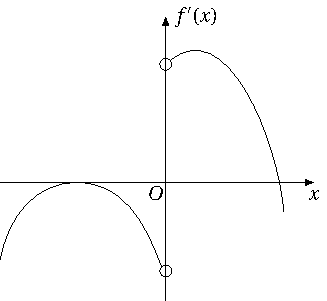
\includegraphics[scale=1]{figure/fig1-2-1.pdf}
			\caption{}\label{fig:1.2.1}
		\end{figure}
	\end{ti}

	\begin{ti}
		当 $x > 0$ 时,曲线 $y = x \sin\frac{1}{x}$ \kuo.
		
		\onech{有且仅有水平渐近线}{有且仅有铅直渐近线}{既有水平渐近线,也有铅直渐近线}{既无水平渐近线,也无铅直渐近线}
	\end{ti}

	\begin{ti}
		曲线 $y = \ln\left( \ee - \frac{1}{x} \right)$ 的全部渐近线为\htwo
		
		\noindent\htwo.
	\end{ti}

	\begin{ti}
		曲线 $y = \ee^{\frac{1}{x^{2}}} \arctan \frac{x^{2} + x + 1}{(x - 1)(x + 2)}$ 的渐近线有\kuo.
		
		\fourch{$1$ 条}{$2$ 条}{$3$ 条}{$4$ 条}
	\end{ti}

	\begin{ti}
		求 $y = \sqrt{4x^{2} + x} \ln\left( 2 + \frac{1}{x} \right)$ 的全部渐近线.
	\end{ti}

	\begin{ti}
		函数 $y = (x - 1)^{2} (x - 2)^{2} (-3 \leq x \leq 4)$ 的值域是
		
		\noindent\htwo.
	\end{ti}

	\begin{ti}
		设正值函数 $f(x)$ 在 $(1,+\infty)$ 内连续,求函数
		\[
			F(x) = \int_{1}^{x} \left[ \left( \frac{2}{x} + \ln x \right) - \left( \frac{2}{t} + \ln t \right) \right] f(t) \dd{t}
		\]
		的最小值点.
	\end{ti}

	\begin{ti}
		函数 $y = x^{x}$ 在区间 $\left[ \frac{1}{\ee},+\infty \right)$ 上\kuo.
		
		\onech{不存在最大值和最小值}{最大值是 $\ee^{\frac{1}{\ee}}$}{最大值是 $\left( \frac{1}{\ee} \right)^{\frac{1}{\ee}}$}{最小值是 $\left( \frac{1}{\ee} \right)^{\frac{1}{\ee}}$}
	\end{ti}

	\begin{ti}
		求函数 $f_{n}(x) = x^{n} \ee^{- n^{2} x}(n = 2,3,\cdots)$ 在 $[0,+\infty)$ 内的最值,并求极限 $\lim_{n \to \infty} f_{n}(x), x \geq 0$.
	\end{ti}

	\begin{ti}
		设 $f(x) = \begin{cases}
			\lim_{n \to \infty} \frac{1}{n} \sum_{k=0}^{n-1} \cos \frac{k}{n}x, & x > 0,\\
			1, & x = 0,\\
			f(-x), & x < 0.
		\end{cases}$
		\begin{enumerate}
			\item 求 $f'(0)$;
			\item 求 $f(x)$ 在 $[-\uppi,\uppi]$ 上的最大值.
		\end{enumerate}
	\end{ti}

	\begin{ti}
		设某物体的温度 $T$ 与时间 $t$ 满足函数关系:
		\[
			T = a\left( 1 - \ee^{-kt} \right) + b,
		\]
		其中 $T$ 的单位是 \si{\degreeCelsius},$t$ 的单位是 \si{min}. 现将该物体放入 \SI{200}{\degreeCelsius} 的高温介质中.
		\begin{enumerate}
			\item 若物体的初始温度是 \SI{20}{\degreeCelsius},求 $a$ 和 $b$;
			\item 若物体温度以 \SI{2}{\degreeCelsius/min} 的速率开始上升,求 $k$.
		\end{enumerate}
	\end{ti}

	\begin{ti}
		曲线 $y = y(x)$ 可表示为 $x = t^{3} - t, y = t^{4} + t$,$t$ 为参数. 证明:
		\begin{enumerate}
			\item $y = y(x)$ 在 $t = 0$ 处为拐点;
			\item $g(x) = \sqrt{\left( \frac{\dd{x}}{\dd{t}} \right)^{2} + \left( \frac{\dd{y}}{\dd{t}} \right)^{2}}$ 在 $t = 0$ 处取得极大值.
		\end{enumerate}
	\end{ti}

	\begin{ti}
		设有曲线弧 $y = \sin x(0 < x < \uppi)$.
		\begin{enumerate}
			\item 求出曲线弧的最小曲率半径;
			\item 求与曲线弧在曲率半径最小的点处相切且具有相同曲率和凹向的抛物线的方程.
		\end{enumerate}
	\end{ti}

	\begin{ti}
		曲线 $2y^{3} - 2y^{2} + 2xy - x^{2} = 1$ 在 $(1,1)$ 处的曲率半径为\htwo.
	\end{ti}

	\begin{ti}
		$y^{2} = 4x$ 在原点处的曲率圆方程为\htwo.
	\end{ti}

	\begin{ti}
		求曲线 $y = \ln x$ 上曲率最大的点,并在该点附近用抛物线 $y = ax^{2} + bx + c$ 近似代替 $y = \ln x$,求 $a,b,c$.
	\end{ti}

	\begin{ti}
		质点 $P$ 沿抛物线 $x = y^{2}(y > 0)$ 移动,$P$ 的横坐标 $x$ 的变化速度 \SI{5}{cm/s}. 当 $x = 9$ 时,点 $P$ 到原点 $O$ 的距离变化速度为\htwo.
	\end{ti}

	\begin{ti}
		半径为 $\frac{1}{2}$ 的圆在抛物线 $x = \sqrt{y}$ 凹的一侧上滚动.
		\begin{enumerate}
			\item 求圆心 $(\xi,\eta)$ 的轨迹方程.
			\item 当圆心以速率 $V_{0}$ 匀速上升时,求圆心的横坐标 $\xi$ 的增长速度.
		\end{enumerate}
	\end{ti}

	\begin{ti}
		球的半径以 \SI{5}{cm/s} 的速度匀速增长,问球的半径为 \SI{50}{cm} 时,球的表面积和体积的增长速度各是多少?
	\end{ti}
	\subsection{中值定理、方程的根、不等式}

	\begin{ti}
		设函数 $f(x)$ 在 $[a,b]$ 上连续,在 $(a,b)$ 内可导,且 $f(a) = f(b) = 0$,求证:
		\begin{enumerate}
			\item 存在 $\xi \in (a,b)$,使 $f(\xi) + \xi f'(\xi) = 0$;
			\item 存在 $\eta \in (a,b)$,使 $\eta f(\eta) + f'(\eta) = 0$.
		\end{enumerate}
	\end{ti}

	\begin{ti}
		设函数 $f(x)$ 在 $[-2,2]$ 上二阶可导,且 $\left| f(x) \right| \leq 1$,又 $f^{2}(0) + \left[ f'(0) \right]^{2} = 4$. 试证:在 $(-2,2)$ 内至少存在一点 $\xi$,使得 $f(\xi) + f''(\xi) = 0$.
	\end{ti}

	\begin{ti}
		设函数 $f(x)$ 在 $[a,b]$ 上连续,在 $(a,b)$ 内可导且 $f(a) \ne f(b)$. 证明:存在 $\xi,\eta \in (a,b)$,使得 $\frac{f'(\xi)}{2\xi} = \frac{f'(\eta)}{b + a}$.
	\end{ti}

	\begin{ti}
		设函数 $f(x)$ 在闭区间 $[a,b]$ 上连续 $(a,b > 0)$,在 $(a,b)$ 内可导. 证明:在 $(a,b)$ 内至少存在一点 $\xi$,使等式 $\frac{1}{a - b} \left| \begin{smallmatrix}
			a & b\\
			f(a) & f(b)
		\end{smallmatrix} \right| = f(\xi) - \xi f'(\xi)$ 成立.
	\end{ti}

	\begin{ti}
		设 $f(x)$ 在闭区间 $[1,2]$ 上可导,证明:存在一点 $\xi \in (1,2)$,使
		\[
			f(2) - 2f(1) = \xi f'(\xi) - f(\xi).
		\]
	\end{ti}

	\begin{ti}
		设 $f(x), g(x)$ 在 $[a,b]$ 上二阶可导,且 $f(a) = f(b) = g(a) = 0$,证明:存在 $\xi \in (a,b)$,使 $f''(\xi) g(\xi) + 2 f'(\xi) g'(\xi) + f(\xi) g''(\xi) = 0$.
	\end{ti}

	\begin{ti}
		设 $f(x)$ 在闭区间 $[-1,1]$ 上具有三阶连续导数,且 $f(-1) = 0$,$f(1) = 1$,$f'(0) = 0$. 证明:在 $[-1,1]$ 内存在 $\xi$,使得 $f'''(\xi) = 3$.
	\end{ti}

	\begin{ti}
		设 $f(x), g(x)$ 在 $[a,b]$ 上二阶可导,$g''(x) \ne 0$,$f(a) = f(b) = g(a) = g(b) = 0$. 证明:
		\begin{enumerate}
			\item 在 $(a,b)$ 内,$g(x) \ne 0$;
			\item 在 $(a,b)$ 内至少存在一点 $\xi$,使 $\frac{f(\xi)}{g(\xi)} = \frac{f''(\xi)}{g''(\xi)}$.
		\end{enumerate}
	\end{ti}

	\begin{ti}
		$f(x)$ 在 $[a,b]$ 上连续,在 $(a,b)$ 内可导,且 $f'(x) \ne 0$. 证明:存在 $\xi, \eta \in (a,b)$,使得
		\[
			\frac{f'(\xi)}{f'(\eta)} = \frac{\ee^{b} - \ee^{a}}{b - a} \ee^{-\eta}.
		\]
	\end{ti}

	\begin{ti}
		设 $f(x)$ 在 $[0,1]$ 上可导,$f(0) = 0$,$\left| f'(x) \right| \leq \left| f(x) \right|$,则 $f(1) = $\htwo.
	\end{ti}

	\begin{ti}
		设 $f(x)$ 在 $[0,4]$ 上一阶可导且 $f'(x) \geq \frac{1}{4}$,$f(2) \geq 0$,则在下列区间上必有 $f(x) \geq \frac{1}{4}$ 成立的是\kuo.

		\fourch{$[0,1]$}{$[1,2]$}{$[2,3]$}{$[3,4]$}
	\end{ti}

	\begin{ti}
		设 $f(x)$ 二阶可导,$f''(x) < 0$,$f'(0) \leq \frac{1}{3}$,$f(0) = 0$,$f(1) = \frac{1}{2}$,并设 $0 < x_{n} < 1$,且 $x_{n+1} = f(x_{n}), n = 1,2,\cdots$.
		\begin{enumerate}
			\item 证明 $\frac{f(x)}{x}$ 在 $(0,+\infty)$ 内单调减少;
			\item 证明 $\lim_{n \to \infty} x_{n}$ 存在.
		\end{enumerate}
	\end{ti}

	\begin{ti}
		设 $\xi_{a}$ 为函数 $f(x) = \arctan x$ 在区间 $[0,a]$ 上使用拉格朗日中值定理时的中值,求 $\lim_{a \to 0^{+}} \frac{\xi_{a}}{a}$.
	\end{ti}

	\begin{ti}
		设函数 $f(x) = \arctan x$,若 $f(x) = f'(\xi) \sin x$,求极限 $\lim_{x \to 0} \frac{\xi^{2}}{x^{2}}$.
	\end{ti}

	\begin{ti}
		设函数 $f(x)$ 在闭区间 $[a,b]$ 上连续,在开区间 $(a,b)$ 内可导,$f'(x) \ne 0$,且 $f(a) = 0$,$f(b) = 2$. 证明在开区间 $(a,b)$ 内存在两个不同的点 $\xi,\eta$,使
		\[
			f'(\eta) \left[ f(\xi) + \xi f'(\xi) \right] = f'(\xi) \left[ b f'(\eta) - 1 \right].
		\]
	\end{ti}

	\begin{ti}
		讨论常数 $a$ 的值,确定曲线 $y = a \ee^{x}$ 与 $y = 1 + x$ 的公共点的个数.
	\end{ti}

	\begin{ti}
		讨论方程 $2x^{3} - 9x^{2} + 12x - a = 0$ 实根的情况.
	\end{ti}

	\begin{ti}
		讨论方程 $a x \ee^{x} + b = 0 (a > 0)$ 实根的情况.
	\end{ti}

	\begin{ti}
		证明:方程 $x^{\alpha} = \ln x (\alpha < 0)$ 在 $(0,+\infty)$ 内有且仅有一个实根.
	\end{ti}

	\begin{ti}
		设 $f(x)$ 可导,证明:$f(x)$ 的两个零点之间一定有 $f(x) + f'(x)$ 的零点.
	\end{ti}

	\begin{ti}
		设 $F(x) = \int_{-1}^{1} |x - t| \ee^{-t^{2}} \dd{t} - \frac{1}{2} \left( \ee^{-1} + 1 \right)$,讨论 $F(x)$ 在区间 $[-1,1]$ 上的零点个数.
	\end{ti}

	\begin{ti}
		证明:当 $x \geq 1$ 时,$\arctan x - \frac{1}{2} \arccos \frac{2x}{1 + x^{2}} \equiv \frac{\uppi}{4}$.
	\end{ti}

	\begin{ti}
		设 $\lim_{x \to 0} \frac{f(x)}{x} = 1$,且 $f''(x) > 0$. 证明:$f(x) \geq x$.
	\end{ti}

	\begin{ti}
		证明:当 $0 < a < b < \uppi$ 时,
		\[
			b \sin b + 2 \cos b + \uppi b > a \sin a + 2 \cos a + \uppi a.
		\]
	\end{ti}

	\begin{ti}
		设 $b > a > \ee$,证明:$a^{b} > b^{a}$.
	\end{ti}

	\begin{ti}
		设一质点在单位时间内由点 $A$ 从静止开始做直线运动至点 $B$ 停止,$A,B$ 两点间距离为 $1$,证明:该质点在 $(0,1)$ 内总有一时刻的加速度的绝对值不小于 $4$.
	\end{ti}

	\begin{ti}
		在区间 $[0,a]$ 上 $\left| f''(x) \right| \leq M$,且 $f(x)$ 在 $(0,a)$ 内取得最大值. 求证:$\left| f'(0) \right| + \left| f'(a) \right| \leq Ma$.
	\end{ti}

	\begin{ti}
		设 $x \in (0,1)$,证明下面不等式
		\begin{enumerate}
			\item $(1 + x) \ln^{2}(1 + x) < x^{2}$;
			\item $\frac{1}{\ln 2} - 1 < \frac{1}{\ln(1 + x)} - \frac{1}{x} < \frac{1}{2}$.
		\end{enumerate}
	\end{ti}

	\begin{ti}
		证明:$\cos \sqrt{2} x \leq - x^{2} + \sqrt{1 + x^{4}}$,其中 $x \in \bigl( 0, \frac{\sqrt{2}\uppi}{4} \bigr)$.
	\end{ti}

	\begin{ti}
		设 $f(x)$ 在 $[a,b]$ 上二阶可导,且 $f'(a) = f'(b) = 0$,证明存在 $\xi \in (a,b)$,使
		\[
			\left| f''(\xi) \right| \geq \frac{4}{(b - a)^{2}} \left| f(b) - f(a) \right|.
		\]
	\end{ti}

	\begin{ti}
		已知 $f(x)$ 二阶可导,且 $f(x) > 0$,$f(x) f''(x) - \bigl[ f'(x) \bigr]^{2} \geq 0 (x \in \mathbb{R})$.
		\begin{enumerate}
			\item 证明 $f(x_{1}) f(x_{2}) \geq f^{2}\left( \frac{x_{1} + x_{2}}{2} \right)(x_{1}, x_{2} \in \mathbb{R})$;
			\item 若 $f(0) = 1$,证明 $f(x) \geq \ee^{f'(0) x} (x \in \mathbb{R})$.
		\end{enumerate}
	\end{ti}

	\begin{ti}
		设 $f(x)$ 在 $[a,b]$ 上具有二阶导数,且 $f''(x) > 0$,证明:
		\[
			f\left( \frac{a + b}{2} \right) < \frac{1}{b - a} \int_{a}^{b} f(t) \dd{t} < \frac{1}{2} \left[ f(a) + f(b) \right].
		\]
	\end{ti}

	\begin{ti}
		证明:$\ee^{x} + \ee^{-x} \geq 2x^{2} + 2 \cos x, -\infty < x < +\infty$.
	\end{ti}

	\begin{ti}
		设 $f(x)$ 在区间 $[0,+\infty)$ 内具有二阶导数,且 $\bigl|f(x)\bigr| \leq 1, 0 < \bigl| f''(x) \bigr| \leq 2 (0 \leq x < +\infty)$. 证明:$\bigl| f'(x) \bigr| \leq 2\sqrt{2}$.
	\end{ti}

	\begin{ti}
		若用 $\frac{2(x - 1)}{x + 1}$ 来近似 $\ln x$,证明当 $x \in [1,2]$ 时,其误差不超过 $\frac{1}{12} (x - 1)^{3}$.
	\end{ti}
	\section{一元函数积分学}
	\subsection{概念与性质}

	\begin{ti}
		设 $f(x)$ 为连续函数,$F(x) = \int_{0}^{x} f(t) \dd{t}$. 试证明:
		\begin{enumerate}
			\item $F(x)$ 的奇偶性正好与 $f(x)$ 的奇偶性相反;
			\item 若 $f(x)$ 为奇函数,则 $f(x)$ 的一切原函数均为偶函数; 若 $f(x)$ 为偶函数,则有且仅有一个原函数为奇函数.
		\end{enumerate}
	\end{ti}

	\begin{ti}
		设 $f(x)$ 在 $(-\infty,+\infty)$ 内连续,以 $T$ 为周期,证明:
		\begin{enumerate}
			\item $\int_{a}^{a + T} f(x) \dd{x} = \int_{0}^{T} f(x) \dd{x}$ ($a$ 为任意实数);
			\item $\int_{0}^{x} f(t) \dd{t}$ 以 $T$ 为周期 $\Longleftrightarrow$ $\int_{0}^{T} f(x) \dd{x} = 0$;
			\item $\int f(x) \dd{x}$ ($f(x)$ 的全体原函数) 周期为 $T$ $\Longleftrightarrow$ $\int_{0}^{T} f(x) \dd{x} = 0$.
		\end{enumerate}
	\end{ti}

	\begin{ti}
		设 $f(x)$ 连续,则在下列变上限积分中,必为偶函数的是\kuo.

		\twoch{$\int_{0}^{x} t \bigl[ f(t) + f(-t) \bigr] \dd{t}$}{$\int_{0}^{x} t \bigl[ f(t) - f(-t) \bigr] \dd{t}$}{$\int_{0}^{x} f\left( t^{2} \right) \dd{t}$}{$\int_{0}^{x} f^{2}(t) \dd{t}$}
	\end{ti}

	\begin{ti}
		设 $F(x) = \int_{x}^{x + 2\uppi} \ee^{\sin t} \dd{t}$,则 $F(x)$ \kuo.

		\twoch{为正常数}{为负常数}{恒为零}{不为常数}
	\end{ti}

	\begin{ti}
		设 $f(x)$ 是以 $l$ 为周期的周期函数,则
		\[
			\int_{a + kl}^{a + (k + 1)l} f(x) \dd{x}
		\]
		的值\kuo.

		\twoch{仅与 $a$ 有关}{仅与 $a$ 无关}{与 $a$ 及 $k$ 都无关}{与 $a$ 及 $k$ 都有关}
	\end{ti}

	\begin{ti}
		设 $f(x)$ 是以 $T$ 为周期的可微函数,则下列函数中以 $T$ 为周期的函数是\kuo.

		\twoch{$\int_{a}^{x} f(t) \dd{t}$}{$\int_{a}^{x} f\bigl( t^{2} \bigr) \dd{t}$}{$\int_{a}^{x} f'\bigl( t^{2} \bigr) \dd{t}$}{$\int_{a}^{x} f(t) f'(t) \dd{t}$}
	\end{ti}

	\begin{ti}
		设 $f(x)$ 是以 $2$ 为周期的连续函数,$G(x) = 2 \int_{0}^{x} f(t) \dd{t} - x \int_{0}^{2} f(t) \dd{t}$,则\kuo.

		\onech{$G(x)$ 是以 $2$ 为周期的周期函数,$G'(x)$ 也是以 $2$ 为周期的周期函数}{$G(x)$ 是以 $2$ 为周期的周期函数,$G'(x)$ 不是以 $2$ 为周期的周期函数}{$G(x)$ 不是以 $2$ 为周期的周期函数,$G'(x)$ 是以 $2$ 为周期的周期函数}{$G(x)$ 不是以 $2$ 为周期的周期函数,$G'(x)$ 也不是以 $2$ 为周期的周期函数}
	\end{ti}

	\begin{ti}
		设 $f(x)$ 可导,且
		\[
			f(x) = x + x \int_{0}^{1} f(x) \dd{x} + x^{2} \lim_{x \to 0} \frac{f(x)}{x},
		\]
		求 $f(x)$.
	\end{ti}

	\begin{ti}
		已知 $f(x)$ 在 $[-1,1]$ 上连续,
		\[
			f(x) = 3x - \sqrt{1 - x^{2}} \int_{0}^{1} f^{2}(x) \dd{x},
		\]
		求 $f(x)$.
	\end{ti}
	\subsection{一元积分比大小}
	
	\begin{ti}
		设 $I_{k} = \int_{0}^{k \uppi} \ee^{x^{2}} \sin x \dd{x} (k = 1,2,3)$,则有\kuo.

		\twoch{$I_{1} < I_{2} < I_{3}$}{$I_{3} < I_{2} < I_{1}$}{$I_{2} < I_{3} < I_{1}$}{$I_{2} < I_{1} < I_{3}$}
	\end{ti}

	\begin{ti}
		设 $N = \int_{-a}^{a} x^{2} \sin^{3}x \dd{x}$,$P = \int_{-a}^{a} \bigl( x^{3} \ee^{x^{2}} - 1 \bigr) \dd{x}$,$Q = \int_{-a}^{a} \cos^{2} x^{3} \dd{x}$,$a \geq 0$,则\kuo.

		\twoch{$N \leq P \leq Q$}{$N \leq Q \leq P$}{$Q \leq P \leq N$}{$P \leq N \leq Q$}
	\end{ti}

	\begin{ti}
		设
		\begin{align*}
			M &= \int_{-\frac{\uppi}{2}}^{\frac{\uppi}{2}} \frac{\sin x}{1 + x^{2}} \cos^{6}x \dd{x},\\
			N &= \int_{-\frac{\uppi}{2}}^{\frac{\uppi}{2}} \bigl( \sin^{3}x + \cos^{6}x \bigr) \dd{x},\\
			P &= \int_{-\frac{\uppi}{2}}^{\frac{\uppi}{2}} \bigl( x^{2} \sin^{3}x - \cos^{6}x \bigr) \dd{x},
		\end{align*}
		则\kuo.

		\twoch{$N < P < M$}{$M < P < N$}{$N < M < P$}{$P < M < N$}
	\end{ti}

	\begin{ti}
		设常数 $\alpha > 0$,积分
		\begin{align*}
			I_{1} &= \int_{0}^{\frac{\uppi}{2}} \frac{\cos x}{1 + x^{\alpha}} \dd{x},\\
			I_{2} &= \int_{0}^{\frac{\uppi}{2}} \frac{\sin x}{1 + x^{\alpha}} \dd{x},
		\end{align*}
		则\kuo.

		\onech{$I_{1} > I_{2}$}{$I_{1} < I_{2}$}{$I_{1} = I_{2}$}{$I_{1}$ 与 $I_{2}$ 的大小与 $\alpha$ 有关}
	\end{ti}

	\begin{ti}
		证明:$\int_{0}^{1} \frac{x \sin \frac{\uppi}{2} x}{1 + x} \dd{x} > \int_{0}^{1} \frac{x \cos \frac{\uppi}{2} x}{1 + x} \dd{x}$
	\end{ti}
	\subsection{定积分定义}

	\begin{ti}
		$\lim_{n \to \infty} \sum_{k=1}^{n} \frac{1}{\sqrt{n^{2} + kn}} = $\hone{4}.
	\end{ti}

	\begin{ti}
		已知 $f(x) = a^{x^{3}}, a > 0$ 且 $a \ne 1$. 求
		\[
			\lim_{n \to \infty} \frac{1}{n^{4}}  \ln \left[ f(1) f(2) \cdots f(n) \right].
		\]
	\end{ti}

	\begin{ti}
		$\lim_{n \to \infty} \frac{\sqrt[n]{(n + 1) (n + 2) \cdots (n + n)}}{n} = $\hone{4}.
	\end{ti}

	\begin{ti}
		$f(x) = \begin{cases}
			\ee^{-x}, & x \ne 0,\\
			\lim_{n \to \infty} 2 \sum_{k=1}^{n} \frac{n}{(n + k)^{2}}, & x = 0,
		\end{cases}$ 求 $f'(0)$.
	\end{ti}

	\begin{ti}
		$\lim_{n \to \infty} \sin \frac{\uppi}{n} \sum_{k=1}^{n} \frac{1}{2 + \cos \frac{k \uppi}{n}} = $\hone{4}.
	\end{ti}

	\begin{ti}
		$\lim_{n \to \infty} \sum_{k=1}^{n} \frac{1}{n + \frac{(k - 1)^{2} + 1}{n}} = $\hone{4}.
	\end{ti}

	\begin{ti}
		$\lim_{n \to \infty} \sum_{k=1}^{n} \frac{3^{\frac{k}{n}}}{n + \frac{1}{k}} = $\hone{4}.
	\end{ti}

	\begin{ti}
		设 $f(x) = \begin{cases}
			\lim_{n \to \infty} \sum_{k=1}^{n} \frac{|x|^{k/n}}{n + \frac{k}{n}}, & x \ne 0,\\
			0, & x = 0,
		\end{cases}$ 求 $f'(x)$.
	\end{ti}
	\subsection{分部积分法}

	\begin{ti}
		求 $\int_{0}^{1} \ln \bigl( x + \sqrt{x^{2} + 3} \bigr) \dd{x}$.
	\end{ti}

	\begin{ti}
		$\int \frac{x \ln ( x + \sqrt{1 + x^{2}} )}{\left( 1 + x^{2} \right)^{2}} \dd{x} = $\htwo.
	\end{ti}

	\begin{ti}
		$\int \frac{x \ln x}{\left( x^{2} - 1 \right)^{\frac{3}{2}}} \dd{x}$.
	\end{ti}

	\begin{ti}
		求 $\int_{-\frac{\uppi}{4}}^{\frac{\uppi}{4}} 5 \cos x \cdot \arctan \ee^{x} \dd{x}$.
	\end{ti}

	\begin{ti}
		求 $\int x \arctan x \dd{x}$.
	\end{ti}

	\begin{ti}
		求 $\int_{0}^{+\infty} \frac{x \ee^{-3x}}{\left( 1 + \ee^{-3x} \right)^{2}} \dd{x}$.
	\end{ti}

	\begin{ti}
		求 $\int_{0}^{1} x \ln (1 - x) \dd{x}$.
	\end{ti}

	\begin{ti}
		设 $f\bigl( \sin^{2}x \bigr) = \frac{x}{\sin x}$,求 $\int \frac{\sqrt{x}}{\sqrt{1 - x}} f(x) \dd{x}$.
	\end{ti}

	\begin{ti}
		已知 $f(x) = \frac{\ee^{x} + \ee^{-x}}{2}$,求 $\int \Bigl[ \frac{f'(x)}{f(x)} + \frac{f(x)}{f'(x)} \Bigr] \dd{x}$.
	\end{ti}

	\begin{ti}
		已知 $\int_{0}^{1} f(x) \dd{x} = 1$,$f(1) = 0$,则 $\int_{0}^{1} x f'(x) \dd{x} = $
		
		\noindent\htwo.
	\end{ti}

	\begin{ti}
		已知 $f(x)$ 的一个原函数为 $(1 + \sin x) \ln x$,求 $\int x f'(x) \dd{x}$.
	\end{ti}

	\begin{ti}
		设 $\frac{\ln x}{x}$ 是 $f(x)$ 的一个原函数,则 $\int_{1}^{\ee} x f'(x) \dd{x} = $
		
		\noindent\htwo.
	\end{ti}

	\begin{ti}
		设 $f(x)$ 有一个原函数 $\frac{\sin x}{x}$,则 $\int_{\frac{\uppi}{2}}^{\uppi} x^{3} f'(x) \dd{x} = $
		
		\noindent\htwo.
	\end{ti}

	\begin{ti}
		设 $f(x) = \lim_{t \to \infty} t^{2} \sin \frac{x}{t} \cdot \bigl[ g\bigl( 2x + \frac{1}{t} \bigr) - g(2x) \bigr]$,$g(x)$ 的一个原函数为 $\ln(x + 1)$,求 $\int_{0}^{1} f(x) \dd{x}$.
	\end{ti}

	\begin{ti}
		设 $f(x)$ 的一个原函数 $F(x) = \ln^{2}\bigl( x + \sqrt{1 + x^{2}} \bigr)$,求 $\int x f'(x) \dd{x}$.
	\end{ti}

	\begin{ti}
		求 $I = \int_{0}^{1} \frac{f(x)}{\sqrt{x}} \dd{x}$,其中 $f(x) = \int_{1}^{\sqrt{x}} \ee^{-t^{2}} \dd{t}$.
	\end{ti}

	\begin{ti}
		设 $f(x) = \int_{0}^{x} \ee^{-t^{2} + 2t} \dd{t}$,求 $\int_{0}^{1} (x - 1)^{2} f(x) \dd{x}$.
	\end{ti}

	\begin{ti}
		设 $y'(x) = \arctan (x - 1)^{2}$,且 $y(0) = 0$,求
		\[
			\int_{0}^{1} y(x) \dd{x}.
		\]
	\end{ti}
	\subsection{换元法}

	\begin{ti}
		求 $\int_{0}^{1} \arcsin \sqrt[3]{x} \dd{x}$.
	\end{ti}

	\begin{ti}
		求 $\int_{0}^{- \ln 2} \sqrt{1 - \ee^{2x}} \dd{x}$.
	\end{ti}

	\begin{ti}
		求 $\int_{0}^{\uppi} \frac{x \sin x}{1 + \sin^{2}x} \dd{x}$.
	\end{ti}

	\begin{ti}
		求 $\int_{0}^{1} \arctan \sqrt{x} \dd{x}$.
	\end{ti}

	\begin{ti}
		求 $\int \frac{\dd{x}}{2 + \cos x}$.
	\end{ti}

	\begin{ti}
		求 $\int_{2}^{+\infty} \frac{\dd{x}}{x \sqrt{x^{2} + 4x}}$.
	\end{ti}

	\begin{ti}
		求 $\int_{0}^{1} \frac{x}{\sqrt{1 - x^{2}}} \arcsin x \dd{x}$.
	\end{ti}

	\begin{ti}
		求 $\int \frac{\dd{x}}{x + \sqrt{x + 2}}$.
	\end{ti}

	\begin{ti}
		求 $\int_{-\frac{\uppi}{4}}^{\frac{\uppi}{4}} \frac{2^{x - 1}}{2^{x} + 1} \cos^{4}2x \dd{x}$.
	\end{ti}

	\begin{ti}
		求 $\int \frac{x + 1}{\left( 1 + x^{2} \right)^{2}} \dd{x}$.
	\end{ti}

	\begin{ti}
		求 $\int \frac{x^{2}}{\sqrt{4 - x^{2}}} \dd{x}$.
	\end{ti}

	\begin{ti}
		求 $\int_{0}^{2} \bigl[ (x - 1)^{3} + 2x \bigr] \sqrt{1 - \cos 2 \uppi x} \dd{x}$.
	\end{ti}

	\begin{ti}
		求 $\int_{0}^{2} (2x + 1) \sqrt{2x - x^{2}} \dd{x}$.
	\end{ti}

	\begin{ti}
		求 $\int_{0}^{4} \frac{3}{4} x^{2} \sqrt{4x - x^{2}} \dd{x}$.
	\end{ti}

	\begin{ti}
		$\int_{-\frac{\uppi}{2}}^{\frac{\uppi}{2}} \frac{3 \ee^{x} \sin^{2}x}{1 + \ee^{x}} \dd{x} = $\hone{4}.
	\end{ti}

	\begin{ti}
		求 $I = \int_{0}^{+\infty} \frac{1}{\left( x^{2} + 1 \right) \left( 1 + x^{5} \right)} \dd{x}$.
	\end{ti}
	\subsection{有理函数积分}

	\begin{ti}
		求 $\int \frac{4x}{(2x + 1)^{3}} \dd{x}$.
	\end{ti}

	\begin{ti}
		求 $\int \frac{x^{3}}{(x - 1)^{100}} \dd{x}$.
	\end{ti}

	\begin{ti}
		求 $\int_{1}^{+\infty} \frac{\dd{x}}{x^{2} (x + 1)}$.
	\end{ti}

	\begin{ti}
		求 $\int \frac{\cos\theta}{\sin\theta - 2 \cos\theta} \dd{\theta}$.
	\end{ti}

	\begin{ti}
		求 $\int \frac{x^{4} + 1}{x \left( x^{2} + 1 \right)^{2}} \dd{x}$.
	\end{ti}

	\begin{ti}
		求 $\int \frac{1}{\ee^{2x} + 3\ee^{x} + 2} \dd{x}$.
	\end{ti}
	\subsection{不可求积可抵消}

	\begin{ti}
		求 $\int \frac{2x + 1}{x^{2}} \ee^{-2x} \dd{x}$.
	\end{ti}

	\begin{ti}
		求 $\int \frac{x + \sin x}{1 + \cos x} \dd{x}$.
	\end{ti}

	\begin{ti}
		求 $\int_{0}^{2} \frac{x \ee^{x}}{(1 + x)^{2}} \dd{x}$.
	\end{ti}

	\begin{ti}
		$\int \ee^{x} \bigl( \frac{1 - x}{1 + x^{2}} \bigr)^{2} \dd{x} = $\htwo.
	\end{ti}
	\subsection{分段函数定积分}

	\begin{ti}
		$\int_{-2}^{2} \max\Bigl\{ x^{2}, \frac{1}{\sqrt[3]{x^{2}}} \Bigr\} \dd{x} = $\hone{4}.
	\end{ti}

	\begin{ti}
		设 $f(x) = \min\bigl\{ (x - k)^{2}, (x - k - 2)^{2} \bigr\}$,$k$ 为任意实数,$g(k) = \int_{0}^{1} f(x) \dd{x}$. 求 $g(k)$ 在 $-2 \leq k \leq 2$ 上的最值.
	\end{ti}
	\subsection{变限积分}
	\paragraph{1. 直接求导}

	\begin{ti}
		设 $f(x)$ 连续,$f(0) = 1$,则曲线 $y = \int_{0}^{x} f(t) \dd{t}$ 在 $(0,0)$ 处的切线方程是\hone{6}.
	\end{ti}

	\begin{ti}
		函数 $F(x) = \int_{1}^{x} \bigl( 1 - \ln \sqrt{t} \bigr) \dd{t} (x > 0)$ 的递减区间为\hone{6}.
	\end{ti}

	\begin{ti}
		设 $f(x)$ 是连续函数,且 $\int_{0}^{x^{3} - 1} f(t) \dd{t} = x$,则 $f(7) = $\hone{4}.
	\end{ti}

	\begin{ti}
		设 $f(x)$ 为连续函数,且 $F(x) = \int_{\frac{1}{x}}^{\ln x} f(t) \dd{t}$,则 $F'(x) = $\hone{6}.
	\end{ti}

	\begin{ti}
		$\frac{\dd}{\dd{x}} \bigl[ \int_{0}^{x} \sin (x - t)^{2} \dd{t} \bigr] = $\hone{6}.
	\end{ti}

	\begin{ti}
		$\lim_{x \to 0} \frac{\int_{0}^{x} \sin^{2}t \dd{t}}{x^{3}} = $\hone{4}.
	\end{ti}

	\begin{ti}
		设 $f(x) = \int_{0}^{\sin x} \sin 2t \dd{t}$,$g(x) = \int_{0}^{2x} \ln(1 + t) \dd{t}$,则当 $x \to 0$ 时,$f(x)$ 与 $g(x)$ 相比是\kuo.

		\twoch{等价无穷小}{同阶但非等价无穷小}{高阶无穷小}{低阶无穷小}
	\end{ti}

	\begin{ti}
		函数 $f(x) = \int_{0}^{x} \frac{1}{x} \bigl( t^{2} - t \bigr) \dd{t} (x > 0)$ 的最小值为
		
		\noindent\kuo.

		\fourch{$-\frac{3}{16}$}{$-1$}{$0$}{$-\frac{1}{2}$}
	\end{ti}

	\begin{ti}
		设函数 $f(x)$ 在 $[a,b]$ 上连续,且 $f(x) > 0$. 则方程 $\int_{a}^{x} f(t) \dd{t} + \int_{b}^{x} \frac{1}{f(t)} \dd{t} = 0$ 在 $(a,b)$ 内的根有\kuo.
		
		\twoch{$0$ 个}{$1$ 个}{$2$ 个}{无穷多个}
	\end{ti}

	\begin{ti}
		设 $f(x)$ 连续,$f(0) = 1$,$f'(0) = 2$,则下列曲线中与曲线 $y = f(x)$ 必有公共切线的是\kuo.

		\twoch{$y = \int_{0}^{x} f(t) \dd{t}$}{$y = 1 + \int_{0}^{x} f(t) \dd{t}$}{$y = \int_{0}^{2x} f(t) \dd{t}$}{$y = 1 + \int_{0}^{2x} f(t) \dd{t}$}
	\end{ti}

	\begin{ti}
		设正值函数 $f(x)$ 在 $[1,+\infty)$ 上连续,求函数
		\[
			F(x) = \int_{1}^{x} \Biggl[ \Biggl( \frac{2}{x} + \ln x \Biggr) - \Biggl( \frac{2}{t} + \ln t \Biggr) \Biggr] f(t) \dd{t}
		\]
		的最小值点.
	\end{ti}

	\begin{ti}
		设 $f(x)$ 在 $x = 0$ 处可导,又
		\[
			g(x) = \begin{cases}
				x + \frac{1}{2}, & x < 0,\\
				\frac{\sin\frac{x}{2}}{x}, & x > 0,
			\end{cases}
		\]
		求
		\[
			I = \lim_{x \to 0} \frac{ x f(x) (1 + x)^{- \frac{x+1}{x}} + g(x) \int_{0}^{2x} \cos t^{2} \dd{t} }{xg(x)}.
		\]
	\end{ti}

	\paragraph{2. 拆分后再求导}

	\begin{ti}
		设 $\varphi(x)$ 在 $[a,b]$ 上连续,且 $\varphi(x) > 0$,则函数 $y = \varPhi(x) = \int_{a}^{b} |x - t| \varphi(t) \dd{t}$\kuo.

		\onech{在 $(a,b)$ 内的图形为凸}{在 $(a,b)$ 内的图形为凹}{在 $(a,b)$ 内有拐点}{在 $(a,b)$ 内有间断点}
	\end{ti}

	\begin{ti}
		设 $|t| \leq 1$,求积分 $I(t) = \int_{-1}^{1} |x - t| \ee^{2x} \dd{x}$ 的最大值.
	\end{ti}

	\paragraph{3. 换元后再求导}

	\begin{ti}
		设 $f(x)$ 连续,则 $\frac{\dd}{\dd{x}} \bigl[ \int_{0}^{x} t f\bigl( x^{2} - t^{2} \bigr) \dd{t} \bigr] = $\hone{2}
		
		\noindent\hone{4}.
	\end{ti}

	\begin{ti}
		设 $f(x)$ 在 $[0,+\infty)$ 上可导,$f(0) = 0$,其反函数为 $g(x)$,若 $\int_{x}^{x + f(x)} g(t - x) \dd{t} = x^{2} \ln(1 + x)$. 求 $f(x)$.
	\end{ti}

	\begin{ti}
		求 $\int_{0}^{x} f(t) g(x - t) \dd{t} (x \geq 0)$,其中,当 $x \geq 0$ 时,$f(x) = x$,且
		\[
			g(x) = \begin{cases}
				\sin x, & 0 \leq x < \frac{\uppi}{2},\\
				0, & x \geq \frac{\uppi}{2}.
			\end{cases}
		\]
	\end{ti}

	\begin{ti}
		设函数 $f(x)$ 连续,且
		\[
			\int_{0}^{x} t f(2x - t) \dd{t} = \frac{1}{2} \arctan x^{2},
		\]
		已知 $f(1) = 1$,求 $\int_{1}^{2} f(x) \dd{x}$.
	\end{ti}
	\subsection{一元积分的复杂与特色计算}

	\begin{ti}
		设 $I_{n} = \int_{0}^{\frac{\uppi}{4}} \tan^{n}x \dd{x}$($n$ 为非负整数),证明:
		\begin{enumerate}
			\item $I_{n} + I_{n-2} = \frac{1}{n - 1} (n \geq 2)$,并由此求 $I_{n}$;
			\item $\frac{1}{2(n + 1)} < I_{n} < \frac{1}{2(n - 1)}$.
		\end{enumerate}
	\end{ti}

	\begin{ti}
		求 $I_{n} = \int_{-1}^{1} \bigl( x^{2} - 1 \bigr)^{n} \dd{x}$.
	\end{ti}

	\begin{ti}
		设 $a_{n} = \int_{0}^{1} x^{n} \sqrt{1 - x^{2}} \dd{x}$,$b_{n} = \int_{0}^{\frac{\uppi}{2}} \sin^{n}t \dd{t}$,则极限 $\lim_{n \to \infty} \frac{n a_{n}}{b_{n}} = $\kuo.

		\fourch{$1$}{$0$}{$-1$}{$\infty$}
	\end{ti}

	\begin{ti}
		求 $\int_{\ee^{-2 n \uppi}}^{1} \Bigl| \bigl[ \cos \bigl( \ln \frac{1}{x} \bigr) \bigr]' \Bigr| \ln \frac{1}{x} \dd{x}$($n$ 为正整数).
	\end{ti}

	\begin{ti}
		设 $a_{n} = \frac{3}{2} \int_{0}^{\frac{n}{n + 1}} x^{n-1} \sqrt{1 + x^{n}} \dd{x}$,则 $\lim_{n \to \infty} n a_{n} = $\hone{1.2}
		
		\noindent\hone{2.8}.
	\end{ti}

	\begin{ti}
		设 $n$ 为正整数,$I_{n} = \int_{0}^{\frac{\uppi}{2}} \frac{\sin 2nx}{\sin x} \dd{x}$.
		\begin{enumerate}
			\item 证明 $I_{n} - I_{n-1} = (-1)^{n-1} \cdot \frac{2}{2n-1} (n \geq 2)$;
			\item 求 $\int_{0}^{\frac{\uppi}{2}} \frac{\sin 6x}{\sin x} \dd{x}$.
		\end{enumerate}
	\end{ti}

	\begin{ti}
		设 $I_{n} = \int_{0}^{\frac{\uppi}{2}} \frac{\sin^{2}nt}{\sin t} \dd{t}$,其中 $n$ 为正整数.
		\begin{enumerate}
			\item 证明 $I_{n} - I_{n-1} = \frac{1}{2n-1}$,并求 $I_{n}$;
			\item 记 $x_{n} = 2I_{n} - \ln n$,证明 $\lim_{n \to \infty} x_{n}$ 存在.
		\end{enumerate}
	\end{ti}

	\begin{ti}
		设函数 $f(x) = x - [x]$,其中 $[x]$ 表示不超过 $x$ 的最大整数,求极限 $\lim_{x \to +\infty} \frac{1}{x} \int_{0}^{x} f(t) \dd{t}$.
	\end{ti}

	\begin{ti}
		设 $x \geq 0$,记 $x$ 到 $2k$ 的最小距离为 $f(x), k = 0,1,2,\cdots$.
		\begin{enumerate}
			\item 证明 $f(x)$ 以 $2$ 为周期;
			\item 求 $\int_{0}^{1} f(nx) \dd{x}$ 的值($n = 1,2,\cdots$).
		\end{enumerate}
	\end{ti}
	\subsection{反常积分判敛与计算}

	\begin{ti}
		设 $a,b > 0$,反常积分 $\int_{0}^{+\infty} \frac{1}{x^{a} (2020 + x)^{b}} \dd{x}$ 收敛,则\kuo.

		\twoch{$a < 1$ 且 $b > 1$}{$a > 1$ 且 $b > 1$}{$a < 1$ 且 $a + b > 1$}{$a > 1$ 且 $a + b > 1$}
	\end{ti}

	\begin{ti}
		设 $a > b > 0$,反常积分 $\int_{0}^{+\infty} \frac{1}{x^{a} + x^{b}} \dd{x}$ 收敛,则
		
		\noindent\kuo.

		\twoch{$a > 1$ 且 $b > 1$}{$a > 1$ 且 $b < 1$}{$a < 1$ 且 $a + b > 1$}{$a < 1$ 且 $b < 1$}
	\end{ti}

	\begin{ti}
		设 $a, b > 0$,反常积分 $\int_{0}^{\frac{\uppi}{2}} \frac{\dd{x}}{\cos^{a}x \sin^{b}x}$ 收敛,则
		
		\noindent\kuo.

		\twoch{$a > 1$ 且 $b > 1$}{$a > 1$ 且 $b < 1$}{$a < 1$ 且 $b > 1$}{$a < 1$ 且 $b < 1$}
	\end{ti}

	\begin{ti}
		设 $a > 0$,$f(x) = \begin{cases}
			\frac{\arctan x}{x^{\frac{a + 1}{2}}}, & 0 < x < 1,\\
			\frac{\ln ( 1 + \sin \frac{1}{x^{a}} )}{x^{b} \ln \cos \frac{1}{x}}, & 1 \leq x < +\infty.
		\end{cases}$ 若 $\int_{0}^{+\infty} f(x) \dd{x}$ 收敛,则\kuo.

		\twoch{$a > 3$ 且 $a + b > 3$}{$a > 3$ 且 $a + b < 3$}{$a < 3$ 且 $a + b > 3$}{$a < 3$ 且 $a + b < 3$}
	\end{ti}

	\begin{ti}
		判别 $\int_{0}^{1} \bigl( 1 - \frac{\sin x}{x} \bigr)^{- \frac{1}{3}} \dd{x}$ 的敛散性.
	\end{ti}

	\begin{ti}
		\begin{enumerate}
			\item 证明
			\[
				I = \int_{2}^{+\infty} \frac{1}{x \ln^{p}x} \dd{x}\begin{cases}
					p > 1 \text{ 时,收敛},\\
					p \leq 1 \text{ 时,发散};
				\end{cases}
			\]
			\item 当 $p > 1$ 时,求出 $I$ 的最小值.
		\end{enumerate}
	\end{ti}

	\begin{ti}
		设 $a, b > 0$,反常积分 $\int_{1}^{+\infty} \frac{1}{x^{a} \ln^{b}x} \dd{x}$ 收敛,则
		
		\noindent\kuo.

		\twoch{$a > 1$ 且 $b > 1$}{$a > 1$ 且 $b < 1$}{$a < 1$ 且 $b > 1$}{$a < 1$ 且 $b < 1$}
	\end{ti}

	\begin{ti}
		判别 $\int_{1}^{+\infty} \bigl[ \ln \bigl( 1 + \frac{1}{x} \bigr) - \frac{1}{1 + x} \bigr] \dd{x}$ 的敛散性.
	\end{ti}

	\begin{ti}
		求反常积分 $\int_{0}^{1} \frac{x^{b} - x^{a}}{\ln x} \dd{x} (a,b > 0)$.
	\end{ti}

	\begin{ti}
		求反常积分
		\[
			\int_{0}^{+\infty} \frac{1}{ \bigl(1 + x^{2}\bigr) \bigl(1 + x^{\alpha}\bigr) } \dd{x} (\alpha \ne 0).
		\]
	\end{ti}

	\begin{ti}
		设 $\lambda \in \mathbb{R}$,求证:
		\[
			\int_{0}^{\frac{\uppi}{2}} \frac{1}{1 + (\tan x)^{\lambda}} \dd{x} = \int_{0}^{\frac{\uppi}{2}} \frac{1}{1 + (\cot x)^{\lambda}} \dd{x} = \frac{\uppi}{4}.
		\]
	\end{ti}

	\begin{ti}
		设
		\[
			f(x) = \begin{cases}
				\frac{ 2 + x (\arcsin x)^{2} }{\sqrt{4 - x^{2}}}, & -1 \leq x \leq 1,\\
				\frac{\arctan x}{x^{2}}, & x > 1,
			\end{cases}
		\]
		求 $\int_{-1}^{+\infty} f(x) \dd{x}$.
	\end{ti}
	\subsection{一元积分的几何应用}

	\begin{ti}
		求曲线 $y = x \sqrt{4x - x^{2}}$ 在 $[0,4]$ 上与 $x$ 轴所围图形绕 $y$ 轴旋转一周所得的旋转体的体积.
	\end{ti}

	\begin{ti}
		求曲线 $y = \sqrt{ x (1 - x)^{9} }$ 在 $[0,1]$ 上与 $x$ 轴所围图形绕 $x$ 轴旋转一周所得的旋转体的体积.
	\end{ti}

	\begin{ti}
		求曲线 $y = \sin^{4}x$ 在 $[0,\uppi]$ 上与 $x$ 轴所围图形绕 $y$ 轴旋转一周所得的旋转体的体积.
	\end{ti}

	\begin{ti}
		设 $a > 0$,$0 < b < 1$,由曲线 $y = \ee^{x}$,直线 $y = 1$ 与直线 $x = ab$ 所围平面区域的面积记为 $S_{1}$,由曲线 $y = \ee^{x}$,直线 $x = ab$ 与直线 $y = \ee^{a}$ 所围平面区域的面积记为 $S_{2}$,若 $S_{1} = S_{2}$,求 $\lim_{a \to 0^{+}} b$.
	\end{ti}

	\begin{ti}
		设 $O$ 为坐标原点,$A(1,0)$,$B(1,1)$,$C(0,1)$,记边长为 $1$ 的正方形 $OABC$ 内位于曲线 $y = x^{2} + t$($t$ 为实数)下方图形的面积为 $S(t)$.
		\begin{enumerate}
			\item 求 $S(t)$ 的表达式;
			\item $S(t)$ 在 $[-1,1]$ 上是否满足拉格朗日中值定理的条件,说明理由.
		\end{enumerate}
	\end{ti}

	\begin{ti}
		设曲线方程为 $y = \ee^{-x}(x \geq 0)$.
		\begin{enumerate}
			\item 曲线 $y = \ee^{-x}$,$x$ 轴,$y$ 轴和直线 $x = \xi(\xi > 0)$ 所围平面图形绕 $x$ 轴旋转一周,得旋转体,求此旋转体体积 $V(\xi)$,以及满足 $V(a) = \frac{1}{2} \lim_{\xi \to +\infty} V(\xi)$ 的 $a$ 值;
			\item 在此曲线上找一点,使过该点的切线与两个坐标轴所夹平面图形的面积最大,并求出该面积.
		\end{enumerate}
	\end{ti}

	\begin{ti}
		设 $n$ 为正整数,$A_{n}$ 是在第一象限内曲线 $y = n \cos nx$ 与该曲线在点 $\bigl( \frac{\uppi}{2n},0 \bigr)$ 处的切线所围成的平面图形的面积. 则\kuo.

		\twoch{$A_{n}$ 与 $n$ 有关}{$A_{n}$ 与 $n$ 无关}{无法判断}{以上结论都不正确}
	\end{ti}

	\begin{ti}
		\begin{enumerate}
			\item 如图~\ref{fig:1.3.1} 所示,设曲线 $L$ 具有如下性质:中间曲线 $y = 2x^{2}$ 上每一点 $P$ 都使得图中 $A$ 的面积等于 $B$ 的面积,求曲线 $L$ 的方程;
			\item 如图~\ref{fig:1.3.1} 所示,若让 $A,B$ 绕 $y$ 轴旋转一周所得的旋转体体积相等,求曲线 $L$ 的方程.
		\end{enumerate}
		\begin{figure}[htbp]
			\centering
			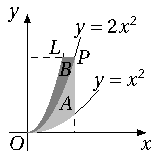
\includegraphics[scale=1]{figure/fig1-3-1.pdf}
			\caption{}\label{fig:1.3.1}
		\end{figure}
	\end{ti}

	\begin{ti}
		如图~\ref{fig:1.3.2} 所示,阴影部分由曲线 $y = \sin x(0 \leq x \leq \uppi)$,直线 $y = a(0 < a < 1)$,$x = \uppi$ 以及 $y$ 轴围成. 此图形绕直线 $y = a$ 旋转一周形成旋转体 $S$. 问 $a$ 为何值时,$S$ 有最小体积,$S$ 有最大体积.
		\begin{figure}[htbp]
			\centering
			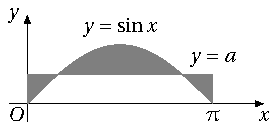
\includegraphics[scale=1]{figure/fig1-3-2.pdf}
			\caption{}\label{fig:1.3.2}
		\end{figure}
	\end{ti}

	\begin{ti}
		求曲线 $y^{2} = \bigl( 1 - x^{2} \bigr)^{3}$ 所围图形的面积.
	\end{ti}

	\begin{ti}
		求曲线 $\sqrt{x} + \sqrt{y} = 1$ 与坐标轴所围图形的面积.
	\end{ti}

	\begin{ti}
		求摆线 $x = t - \sin t$,$y = 1 - \cos t$ 的一拱与 $x$ 轴围成的图形的面积.
	\end{ti}

	\begin{ti}
		求星形线 $x = \cos^{3}t$,$y = \sin^{3}t$ 所围图形的面积.
	\end{ti}

	\begin{ti}
		求阿基米德螺线 $r = a \theta$ 的第一圈与极轴所围图形的面积.
	\end{ti}

	\begin{ti}
		求 $r = \sqrt{2} \sin \theta$ 及 $r^{2} = \cos 2 \theta$ 围成图形公共部分的面积.
	\end{ti}

	\begin{ti}
		求曲线 $y = \frac{1}{x^{2} + 1}$ 和 $x$ 轴之间区域的面积.
	\end{ti}

	\begin{ti}
		求曲线 $y = x \ee^{-\frac{x^{2}}{2}}$ 与其渐近线之间的面积.
	\end{ti}

	\begin{ti}
		记 $l_{1}$ 为椭圆 $x^{2} + 2y^{2} = 2$ 的周长,$l_{2}$ 为曲线 $y_{1} = \sin x$ 在 $0 \leq x \leq 2\uppi$ 上的弧长,$l_{3}$ 为曲线 $y_{2} = \frac{1}{2} \sin 2x$ 在 $0 \leq x \leq 2\uppi$ 上的弧长,则\kuo.

		\twoch{$l_{1} > l_{2} = l_{3}$}{$l_{1} = l_{2} < l_{3}$}{$l_{2} > l_{3} = l_{1}$}{$l_{1} = l_{2} = l_{3}$}
	\end{ti}

	\begin{ti}
		曲线 $\begin{cases}
			x = 3 (t - \sin t)\\
			y = 3 (1 - \cos t)
		\end{cases} (0 \leq t \leq 2\uppi)$ 的弧长为\htwo.
	\end{ti}

	\begin{ti}
		求抛物线 $6y = x^{2}$ 从点 $(0,0)$ 到点 $\bigl( 4,\frac{8}{3} \bigr)$ 之间的弧长.
	\end{ti}

	\begin{ti}
		求星形线 $x = \cos^{3}t$,$y = \sin^{3}t$ 的全长.
	\end{ti}

	\begin{ti}
		在摆线 $x = t - \sin t$,$y = 1 - \cos t$ 上求一点,将摆线第一拱的弧长分为 \ratio{$1$}{$3$}.
	\end{ti}

	\begin{ti}
		求心形线 $r = a (1 + \cos \theta)$ 的全长.
	\end{ti}

	\begin{ti}
		求曲线 $r \theta = 1$ 自 $\theta = \frac{3}{4}$ 至 $\theta = \frac{4}{3}$ 一段的弧长.
	\end{ti}

	\begin{ti}
		求曲线 $y = \int_{0}^{x} \sqrt{\cos t} \dd{t}$ 的全长.
	\end{ti}

	\begin{ti}
		当 $x \geq 0$ 时,曲线 $y = \frac{1}{4} \int_{0}^{2} x \sqrt{12 - x^{2} t^{2}} \dd{t}$ 的全长为\htwo.
	\end{ti}

	\begin{ti}
		设函数 $y = f(x)$ 在区间 $[0,1]$ 上非负、存在二阶导数,且 $f(0) = 0$,有一块质量均匀的平板 $D$,其占据的区域是曲线 $y = f(x)$ 与直线 $x = 1$ 以及 $x$ 轴围成的平面图形(图~\ref{fig:1.3.3}). 用 $\overline{x}$ 表示平板 $D$ 的质心的横坐标. 求证:
		\begin{enumerate}
			\item 若 $f'(x) > 0(0 \leq x \leq 1)$,则 $\overline{x} > \frac{1}{2}$(如图~\ref{fig:1.3.3:a});
			\item 若 $f''(x) > 0(0 \leq x \leq 1)$,则 $\overline{x} > \frac{2}{3}$(如图~\ref{fig:1.3.3:b}).
		\end{enumerate}
		\begin{figure}[htbp]
			\begin{floatrow}
			  \ffigbox[\textwidth]{
				\begin{subfloatrow}[2]
				  \ffigbox[\FBwidth]{
					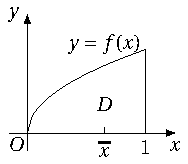
\includegraphics[scale=1]{figure/fig1-3-3-a.pdf}
				  }{\caption{}\label{fig:1.3.3:a}}
				  \ffigbox[\FBwidth]{
					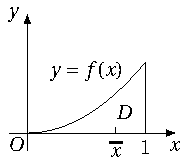
\includegraphics[scale=1]{figure/fig1-3-3-b.pdf}
				  }{\caption{}\label{fig:1.3.3:b}}
				\end{subfloatrow}
			  }{\caption{}\label{fig:1.3.3}}
			\end{floatrow}
		  \end{figure}
	\end{ti}

	\begin{ti}
		求由曲线 $y^{2} = x^{3} - x^{4}$ 所围成的平面图形的形心.
	\end{ti}

	\begin{ti}
		求由曲线 $y = x^{2}$ 与直线 $y = x$ 在第一象限内所围成的图形绕该直线旋转所成立体的体积.
	\end{ti}
	\subsection{一元积分的物理应用}

	\begin{ti}
		水从一根底面半径为 \SI{1}{cm} 的圆柱形管道中流出.因为水有黏性,在流动过程中受到管道壁的阻滞,所以流动的速度是随着到管道中心的距离而变化的. 距管道中心越远,水流速度越小. 在距离管道中心 $r$ \si{cm} 处的水的流动速度为 $10 \bigl(1 - r^{2}\bigr)$ \si{cm/s}. 问水是以多大流量(以 \si{cm^{3}/s} 为单位)流过管道的?
	\end{ti}

	\begin{ti}
		某城市的人口密度近似为 $p(r) = \frac{4}{r^{2} + 20}$,$p(r)$ 表示距市中心 $r$ \si{km} 区域的人口数,单位为每平方千米 $10$ 万人.
		\begin{enumerate}
			\item 试求距市中心 \SI{2}{km} 区域内的人口数;
			\item 若人口密度近似为 $p(r) = 1.2 \ee^{-0.2r}$ 单位不变,试求距市中心 \SI{2}{km} 区域内的人口数.
		\end{enumerate}
	\end{ti}

	\begin{ti}
		半径为 $1$ 的球沉入水中,球的上顶与水平面齐平. 球与水的密度相同记为 $\rho$,重力加速度记为 $g$,现将球打捞出水,至少需做多少功?
	\end{ti}

	\begin{ti}
		一个均质的物体,高 \SI{4}{m},水平截面面积是高度 $h$ (从底部算起)的函数 $S = 20 + 3h^{2}$. 已知物体的密度与水的密度同为 \SI{e3}{kg/m^3},此物体沉在水中,上表面与水面平齐,问将此物体打捞出水,至少需做功多少(设重力加速度 $g = $ \SI{10}{m/s^2})?
	\end{ti}

	\begin{ti}
		一块 \SI{1000}{kg} 的冰块要被吊起 \SI{30}{m} 高,而这块冰以 \SI{0.02}{kg/s} 的速度溶化,假设冰块以 \SI{0.1}{m/s} 的速度被吊起,吊索的线密度为 \SI{4}{kg/m}. 求把这块冰吊到指定高度需作的功(设重力加速度 $g = $ \SI{10}{m/s^2}).
	\end{ti}

	\begin{ti}
		\begin{enumerate}
			\item 宽度为 \SI{6}{m} 的金属板,三分之一作为侧边,做成排水沟(如图~\ref{fig:1.3.4}). 问折起角度多大时,排水沟的截面积 $S$ 最大;\label{3.142:1}
			\begin{figure}[htbp]
				\centering
				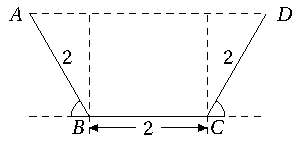
\includegraphics[scale=1]{figure/fig1-3-4.pdf}
				\caption{}\label{fig:1.3.4}
			\end{figure}
			\item 设一抛物线过(\ref{3.142:1})中所求得截面的 $A,D$ 及 $BC$ 中点,记该抛物线与直线段 $AD$ 所围成封闭平面的面积 $\widetilde{S}$,求 $\frac{S}{\widetilde{S}}$;\label{3.142:2}
			\item 若排水沟长为 \SI{1}{m},其横截面原为(\ref{3.142:1})中等腰梯形的形状,因淤泥沉积形成了(\ref{3.142:2})中抛物线的形状. 现清除淤泥,恢复(\ref{3.142:1})中的形状,将淤泥搬运出排水沟,则至少作多少功?(设单位体积的淤泥重为 $\rho$ \si{N/m^3})
		\end{enumerate}
	\end{ti}
	\subsection{平均值}

	\begin{ti}
		$f(x) = \int_{x}^{1} \cos t^{2} \dd{t}$ 在区间 $[0,1]$ 上的平均值为\htwo.
	\end{ti}

	\begin{ti}
		某质点以速度 $v = 3t^{2} + 2t$(\si{m/s})做直线运动,则它在 $t = 0$ 到 $t = $\SI{3}{s} 这段时间上的平均速度为\htwo.
	\end{ti}
	\subsection{一元积分不等式}

	\begin{ti}
		已知函数 $f(x)$ 在区间 $[a,b]$ 上连续并单调增加,求证:
		\[
			\int_{a}^{b} \Biggl( \frac{b - x}{b - a} \Biggr)^{n} f(x) \dd{x} \leq \frac{1}{n + 1} \int_{a}^{b} f(x) \dd{x} (n \in \mathbb N).
		\]
	\end{ti}

	\begin{ti}
		设 $f(x)$ 在 $[a,b]$ 上连续,且 $f(x) > 0$,证明:
		\[
			\ln \left[ \frac{1}{b - a} \int_{a}^{b} f(x) \dd{x} \right] \geq \frac{1}{b - a} \int_{a}^{b} \ln f(x) \dd{x}.
		\]
	\end{ti}

	\begin{ti}
		设 $f(x)$ 二阶可导,$f''(x) \geq 0$,$g(x)$ 为连续函数,若 $a > 0$,求证:
		\[
			\frac{1}{a} \int_{0}^{a} f\bigl[g(x)\bigr] \dd{x} \geq f\left[ \frac{1}{a} \int_{0}^{a} g(x) \dd{x} \right].
		\]
	\end{ti}

	\begin{ti}
		设 $f(x)$ 在闭区间 $[0,1]$ 上有二阶导数,且 $f\bigl( \frac{1}{2} \bigr) = 1$,$f''(x) > 0$,证明 $\int_{0}^{1} f(x) \dd{x} \geq 1$.
	\end{ti}

	\begin{ti}
		\begin{enumerate}
			\item 证明不等式
			\[
				\ln(n+1) < 1 + \frac{1}{2} + \frac{1}{3} + \cdots + \frac{1}{n} < 1 + \ln n;
			\]
			\item 证明数列 $a_{n} = 1 + \frac{1}{2} + \frac{1}{3} + \cdots + \frac{1}{n} - \ln(n+1)$ 单调增加,且 $0 < a_{n} < 1$.
		\end{enumerate}
	\end{ti}

	\begin{ti}
		当 $x \geq 0$ 时,在曲线 $y = \ee^{-2x}$ 上面作一个台阶曲线,台阶的宽度皆为 $1$(如图~\ref{fig:1.3.5}). 求图中无穷多个阴影部分的面积之和 $S$.
		\begin{figure}[htbp]
			\centering
			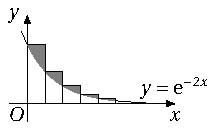
\includegraphics[scale=1]{figure/fig1-3-5.pdf}
			\caption{}\label{fig:1.3.5}
		\end{figure}
	\end{ti}

	\begin{ti}
		求极限 $\lim_{n \to \infty} \frac{\sum_{k=1}^{n} \frac{1}{k}}{\ln n}$.
	\end{ti}
	\section{多元函数微分学}
	\subsection{概念}

	\begin{ti}
		设 $f(x,y) = \ee^{x + y} \Bigl[ x^{\frac{1}{3}} (y - 1)^{\frac{1}{3}} + y^{\frac{1}{3}} (x - 1)^{\frac{2}{3}} \Bigr]$,则在点 $(0,1)$ 处的两个偏导数 $f_{x}'(0,1)$ 和 $f_{y}'(0,1)$ 的情况为\kuo.

		\onech{两个偏导数均不存在}{$f_{x}'(0,1)$ 不存在,$f_{y}'(0,1) = \frac{4}{3}\ee$}{$f_{x}'(0,1) = \frac{\ee}{3}$,$f_{y}'(0,1) = \frac{4}{3}\ee$}{$f_{x}'(0,1) = \frac{\ee}{3}$,$f_{y}'(0,1)$ 不存在}
	\end{ti}

	\begin{ti}
		函数 $z = f(x,y) = \sqrt{|xy|}$ 在点 $(0,0)$ \kuo.

		\onech{连续,但偏导数不存在}{偏导数存在,但不可微}{可微}{偏导数存在且连续}
	\end{ti}

	\begin{ti}
		函数 $f(x,y) = \sqrt[3]{x^{2} y}$ 在点 $(0,0)$ 处:
		\begin{enumerate}
			\item 是否连续,说明理由;
			\item 偏导数是否存在,说明理由;
			\item 是否可微,说明理由.
		\end{enumerate}
	\end{ti}

	\begin{ti}
		设
		\begin{enumerate}
			\item $f(x,y) = \begin{cases}
				\frac{x^{2} y^{2}}{\left( x^{2} + y^{2} \right)^{3/2}}, & (x,y) \ne (0,0),\\
				0, & (x,y) = (0,0);
			\end{cases}$
			\item $g(x,y) = \begin{cases}
				\bigl( x^{2} + y^{2} \bigr) \sin \frac{1}{x^{2} + y^{2}}, & (x,y) \ne (0,0),\\
				0, & (x,y) = (0,0).
			\end{cases}$
		\end{enumerate}
		讨论它们在点 $(0,0)$ 处的
		\begin{enumerate}
			\item[\libcirc{1}] 偏导数的存在性;
			\item[\libcirc{2}] 函数的连续性;
			\item[\libcirc{3}] 方向导数的存在性;
			\item[\libcirc{4}] 函数的可微性.
		\end{enumerate}
	\end{ti}

	\begin{ti}
		已知 $f(x,y) = \bigl( xy + xy^{2} \bigr) \ee^{x + y}$,则 $\frac{\partial^{10}f}{\partial x^{5} \partial y^{5}} = $\htwo.
	\end{ti}

	\begin{ti}
		\begin{enumerate}
			\item 设 $y = \frac{1}{x(1 - x)}$,求 $\frac{\dd^{n}y}{\dd{x^{n}}}$;
			\item 设 $z = \frac{y^{2}}{x(1 - x)}$,求 $\frac{\partial^{n}z}{\partial x^{n}}$.
		\end{enumerate}
	\end{ti}

	\begin{ti}
		设 $z = y^{2} \ln \bigl( 1 - x^{2} \bigr)$,求 $\frac{\partial^{n}z}{\partial x^{n}}$.
	\end{ti}

	\begin{ti}
		设 $z = x \ln \bigl[ \bigl( 1 + y^{2} \bigr) \ee^{x^{2} \sin y} \bigr]$,则 $\frac{\partial^{4}z}{\partial y^{2} \partial x^{2}} = $\htwo.
	\end{ti}

	\begin{ti}
		设函数 $f(x,y)$ 的一阶偏导数连续,在点 $(1,0)$ 的某邻域内有
		\[
			f(x,y) = 1 - x - 2y + o\left( \sqrt{(x - 1)^{2} + y^{2}} \right)
		\]
		成立. 记 $z(x,y) = f\bigl( \ee^{y}, x + y \bigr)$,则 $\dd{[z(x,y)]}|_{(0,0)} = $\htwo.
	\end{ti}

	\begin{ti}
		设函数 $f(x,y)$ 及它的二阶偏导数在全平面连续,且 $f(0,0) = 0$,$\Bigl| \frac{\partial f}{\partial x} \Bigr| \leq 2 \bigl|x - y\bigr|$,$\Bigl| \frac{\partial f}{\partial y} \Bigr| \leq 2 \bigl|x - y\bigr|$. 求证:$\bigl|f(5,4)\bigr| \leq 1$.
	\end{ti}

	\begin{ti}
		二元函数 $f(x,y) = x^{y}$ 在点 $(\ee,0)$ 处的二阶(即 $n = 2$) 泰勒展开式(不要求写出余项)为\htwo.
	\end{ti}
	\subsection{多元微分法}

	\begin{ti}
		设 $F(u,v)$ 对其变元 $u,v$ 具有二阶连续偏导数,并设 $z = F\bigl( \frac{y}{x},x^{2} + y^{2} \bigr)$,则 $\frac{\partial^{2}z}{\partial x \partial y} = $\htwo.
	\end{ti}

	\begin{ti}
		设 $u = y f \bigl( \frac{x}{y} \bigr) + x g \bigl( \frac{y}{x} \bigr)$,其中函数 $f,g$ 具有二阶连续偏导数,求 $x \frac{\partial^{2}u}{\partial x^{2}} + y \frac{\partial^{2}u}{\partial x \partial y}$.
	\end{ti}

	\begin{ti}
		设函数 $z = f(u)$,方程 $u = \varphi(u) + \int_{y}^{x} P(t) \dd{t}$ 确定 $u$ 是 $x,y$ 的函数,其中 $f(u),\varphi(u)$ 可微,$P(t),\varphi'(u)$ 连续,且 $\varphi'(u) \ne 1$. 求 $P(y) \frac{\partial z}{\partial x} + P(x) \frac{\partial z}{\partial y}$.
	\end{ti}

	\begin{ti}
		设 $f(x,y) = \int_{0}^{xy} \ee^{-t^{2}} \dd{t}$,求 $\frac{x}{y} \cdot \frac{\partial^{2}f}{\partial x^{2}} - 2 \frac{\partial^{2}f}{\partial x \partial y} + \frac{y}{x} \cdot \frac{\partial^{2}f}{\partial y^{2}}$.
	\end{ti}

	\begin{ti}
		设函数 $f(x,y)$ 可微,又 $f(0,0) = 0$,$f_{x}'(0,0) = a$,$f_{y}'(0,0) = b$,且 $\varphi(t) = f \bigl[ t, f \bigl( t, t^{2} \bigr) \bigr]$,求 $\varphi'(0)$.
	\end{ti}

	\begin{ti}
		设函数 $u = u(x,y)$ 满足 $\frac{\partial^{2}u}{\partial x^{2}} = \frac{\partial^{2}u}{\partial y^{2}}$ 及
		\[
			u(x,2x) = x,u_{1}'(x,2x) = x^{2},
		\]
		$u$ 有二阶连续偏导数,则 $u_{11}''(x,2x) = $\kuo.

		\fourch{$\frac{4}{3}x$}{$-\frac{4}{3}x$}{$\frac{3}{4}x$}{$-\frac{3}{4}x$}
	\end{ti}

	\begin{ti}
		若函数 $u = x y f \bigl( \frac{x + y}{xy} \bigr)$,其中 $f$ 是可微函数,且 $x^{2} \frac{\partial u}{\partial x} - y^{2} \frac{\partial u}{\partial y} = G(x,y) u$,则函数 $G(x,y) = $\kuo.

		\fourch{$x + y$}{$x - y$}{$x^{2} - y^{2}$}{$(x + y)^{2}$}
	\end{ti}

	\begin{ti}
		设函数 $u = f \bigl( \ln \sqrt{x^{2} + y^{2}} \bigr)$,满足 $\frac{\partial^{2}u}{\partial x^{2}} + \frac{\partial^{2}u}{\partial y^{2}} = \bigl( x^{2} + y^{2} \bigr)^{\frac{3}{2}}$,且极限
		\[
			\lim_{x \to 0} \frac{\int_{0}^{1} f(xt) \dd{t}}{x} = -1,
		\]
		试求函数 $f(x)$ 的表达式.
	\end{ti}

	\begin{ti}
		设 $u(x,y)$ 连续,证明无零值的函数 $u(x,y)$ 可分离变量(即 $u(x,y) = f(x) \cdot g(y)$)的充分必要条件是
		\[
			u \frac{\partial^{2}u}{\partial x \partial y} = \frac{\partial u}{\partial x} \frac{\partial u}{\partial y}.
		\]
	\end{ti}

	\begin{ti}
		设 $u = f(x,y,z)$ 有连续偏导数,$y = y(x)$ 和 $z = z(x)$ 分别由方程 $\ee^{xy} - y = 0$ 和 $\ee^{z} - xz = 0$ 所确定,求 $\frac{\dd{u}}{\dd{x}}$.
	\end{ti}

	\begin{ti}
		已知函数 $F(u,v,w)$ 可微,
		\[
			F_{u}'(0,0,0) = 1,
			F_{v}'(0,0,0) = 2,
			F_{w}'(0,0,0) = 3,
		\]
		函数 $z = f(x,y)$ 由 $F \bigl( 2x - y + 3z, 4x^{2} - y^{2} + z^{2}, xyz \bigr) = 0$ 确定,且满足 $f(1,2) = 0$,则 $f_{x}'(1,2) = $\htwo.
	\end{ti}

	\begin{ti}
		设 $u = f(x,y,z)$,$\varphi\bigl( x^{2},\ee^{y},z \bigr) = 0$,$y = \sin x$,其中 $f,\varphi$ 具有一阶连续的偏导数,且 $\frac{\partial \varphi}{\partial z} \ne 0$,求 $\frac{\dd{u}}{\dd{x}}$.
	\end{ti}

	\begin{ti}
		已知 $\begin{cases}
			z = x^{2} + y^{2},\\
			x^{2} + 2y^{2} + 3z^{2} = 20,
		\end{cases}$ 求 $\frac{\dd{y}}{\dd{x}},\frac{\dd{z}}{\dd{x}}$.
	\end{ti}

	\begin{ti}
		利用变量代换 $u = x$,$v = \frac{y}{x}$,可将方程
		\[
			x \frac{\partial z}{\partial x} + y \frac{\partial z}{\partial y} = z
		\]
		化成新方程\kuo.

		\twoch{$u \frac{\partial z}{\partial u} = z$}{$v \frac{\partial z}{\partial v} = z$}{$u \frac{\partial z}{\partial v} = z$}{$v \frac{\partial z}{\partial u} = z$}
	\end{ti}

	\begin{ti}
		已知函数 $u = u(x,y)$ 满足方程 $\frac{\partial^{2}u}{\partial x^{2}} - \frac{\partial^{2}u}{\partial y^{2}} + k \bigl( \frac{\partial u}{\partial x} + \frac{\partial u}{\partial y} \bigr) = 0$. 试确定参数 $a,b$,利用变换 $u(x,y) = v(x,y) \ee^{ax + by}$ 将原方程变形,使新方程中不含有一阶偏导数项.
	\end{ti}

	\begin{ti}
		设 $A,B,C$ 为常数,$B^{2} - AC > 0$,$A \ne 0$,$u(x,y)$ 具有二阶连续偏导数. 证明:必存在非奇异线性变换
		\[
			\xi = \lambda_{1}x + y, \eta = \lambda_{2}x + y(\lambda_{1},\lambda_{2} \text{ 为常数}),
		\]
		将方程 $A \frac{\partial^{2}u}{\partial x^{2}} + 2B \frac{\partial^{2}u}{\partial x \partial y} + C \frac{\partial^{2}u}{\partial y^{2}} = 0$ 化成 $\frac{\partial^{2}u}{\partial \xi \partial \eta} = 0$.
	\end{ti}

	\begin{ti}
		设 $h(t)$ 为三阶可导函数,$u = h(xyz)$,$h(1) = f_{xy}''(0,0)$,$h'(1) = f_{yx}''(0,0)$,且满足
		\[
			\frac{\partial^{3}u}{\partial x \partial y \partial z} = x^{2} y^{2} z^{2} h'''(xyz),
		\]
		求 $u$ 的表达式,其中
		\[
			f(x,y) = \begin{cases}
				x y \frac{x^{2} - y^{2}}{x^{2} + y^{2}}, & (x,y) \ne (0,0)\\
				0, & (x,y) = (0,0).
			\end{cases}
		\]
	\end{ti}

	\begin{ti}
		设 $z = z(u,v)$ 具有二阶连续偏导数,且 $z = z(x + y, x - y)$ 满足微分方程
		\[
			\frac{\partial^{2}z}{\partial x^{2}} + 2 \frac{\partial^{2}z}{\partial x \partial y} + \frac{\partial^{2}z}{\partial y^{2}} = 1.
		\]
		\begin{enumerate}
			\item 求 $z = z(u,v)$ 所满足关于 $u,v$ 的微分方程;\label{4.29:1}
			\item 由(\ref{4.29:1})求出 $z = z(x + y, x - y)$ 的一般表达式.
		\end{enumerate}
	\end{ti}

	\begin{ti}
		设 $f(u,v)$ 可微,证明曲面 $f(ax - bz, ay - cz) = 0$ 上任一点的切平面都与某一定直线平行,其中 $a,b,c$ 是不同时为零的常数.
	\end{ti}

	\begin{ti}
		证明曲面 $\ee^{2x - z} = f \bigl( \uppi y - \sqrt{2}z \bigr)$ 是柱面,其中 $f$ 可微.
	\end{ti}
	\subsection{多元函数的极值、最值问题}

	\begin{ti}
		函数
		\[
			f(x,y) = \begin{cases}
				\frac{\sin ( x^{2} + y^{2} )}{x^{2} + y^{2}}, & (x,y) \ne (0,0),\\
				1, & (x,y) = (0,0)
			\end{cases}
		\]
		在 $D = \bigl\{ (x,y) \bigl| x^{2} + y^{2} \leq 1 \bigr\}$ 上\kuo.

		\onech{有最大值,无最小值}{有最小值,无最大值}{既无最大值,又无最小值}{既有最大值,又有最小值}
	\end{ti}

	\begin{ti}
		设 $f(x,y)$ 在点 $(0,0)$ 的邻域内连续,且
		\[
			\lim_{(x,y) \to (0,0)} \frac{f(x,y) - 4xy}{x^{2} + y^{2}} = 1,
		\]
		则\kuo.

		\onech{点 $(0,0)$ 是 $f(x,y)$ 的极小值点}{点 $(0,0)$ 是 $f(x,y)$ 的极大值点}{点 $(0,0)$ 不是 $f(x,y)$ 的极值点}{所给条件不足以判断点 $(0,0)$ 是否为 $f(x,y)$ 的极值点}
	\end{ti}

	\begin{ti}
		设 $f(x,y)$ 是连续函数,且 $\lim_{\substack{x \to 0\\ y \to 0}} \frac{f(x,y) - f(0,0)}{x^{3} + y^{3} - 3x^{2} - 3y^{2}} = 1$,则\kuo.

		\onech{$f(0,0)$ 为 $f(x,y)$ 的极大值}{$f(0,0)$ 为 $f(x,y)$ 的极小值}{$f(0,0)$ 不是 $f(x,y)$ 的极值}{不能确定}
	\end{ti}

	\begin{ti}
		已知函数 $f(x,y)$ 在点 $(0,0)$ 的某邻域内连续,且
		\[
			\lim_{\substack{x \to 0\\ y \to 0}} \frac{f(x,y) - axy}{\bigl( x^{2} + y^{2} \bigr)^{2}} = 1,
		\]
		其中 $a$ 为非零常数,则 $f(0,0)$\kuo.

		\twoch{是极大值}{是极小值}{不是极值}{是否取极值与 $a$ 有关}
	\end{ti}

	\begin{ti}
		设 $f(x,y)$ 在点 $O(0,0)$ 的某邻域 $U$ 内连续,且 $\lim_{(x,y) \to (0,0)} \frac{f(x,y) - xy}{x^{2} + y^{2}} = a$,常数 $a > \frac{1}{2}$. 试讨论 $f(0,0)$ 是否为 $f(x,y)$ 的极值?若是极值,判断是极大值还是极小值?
	\end{ti}

	\begin{ti}
		设 $u(x,y)$ 在平面有界闭区域 $D$ 上具有二阶连续偏导数,且
		\[
			\frac{\partial^{2}u}{\partial x \partial y} \ne 0,\frac{\partial^{2}u}{\partial x^{2}} \cdot \frac{\partial^{2}u}{\partial y^{2}} = 0,
		\]
		则 $u(x,y)$ 的\kuo.

		\onech{最大值点和最小值点必定都在 $D$ 的内部}{最大值点和最小值点必定都在 $D$ 的边界上}{最大值点在 $D$ 的内部,最小值点在 $D$ 的边界上}{最小值点在 $D$ 的内部,最大值点在 $D$ 的边界上}
	\end{ti}

	\begin{ti}
		已知函数 $z = z(x,y)$ 在区域 $D$ 内满足方程 $\frac{\partial^{2}z}{\partial x^{2}} \cdot \frac{\partial^{2}z}{\partial y^{2}} + a \frac{\partial z}{\partial x} + b \frac{\partial z}{\partial y} + c = 0$(常数 $c > 0$),则在 $D$ 内函数 $z = z(x,y)$\kuo.

		\twoch{存在极大值}{存在极小值}{无极值}{无法判断}
	\end{ti}

	\begin{ti}
		函数 $z = x^{3} + y^{3} - 3x^{2} - 3y^{2}$ 的极小值点是\kuo.

		\fourch{$(0,0)$}{$(2,2)$}{$(0,2)$}{$(2,0)$}
	\end{ti}

	\begin{ti}
		若函数 $z = 2x^{2} + 2y^{2} + 3xy + ax + by + c$ 在点 $(-2,3)$ 处取得极小值 $-3$,则 $abc = $\htwo.
	\end{ti}

	\begin{ti}
		设函数 $z = z(x,y)$ 是由方程
		\[
			x^{2} - 6xy + 10y^{2} - 2yz - z^{2} + 32 = 0
		\]
		确定,讨论函数 $z(x,y)$ 的极大值与极小值.
	\end{ti}

	\begin{ti}
		函数 $f(x,y) = \ee^{-x} \bigl( ax + b - y^{2} \bigr)$,若 $f(-1,0)$ 为其极大值,则 $a,b$ 满足\htwo.
	\end{ti}

	\begin{ti}
		已知矩形的周长为 $2p$,将它绕其中一边旋转一周而构成一旋转体(圆柱体),求该圆柱体的半径与高各为多少时,该圆柱体体积最大?
	\end{ti}

	\begin{ti}
		\begin{enumerate}
			\item 设 $x > 0$,$y > 0$,$z > 0$,求函数 $f(x,y,z) = x y z^{3}$ 在约束条件 $x^{2} + y^{2} + z^{2} = 5 R^{2}$($R > 0$ 为常数)下的最大值;\label{4.44:1}
			\item 由(\ref{4.44:1})的结论证明:当 $a > 0$,$b > 0$,$c > 0$ 时,
			\[
				a b c^{3} \leq 27 \Biggl( \frac{a + b + c}{5} \Biggr)^{5}.
			\]
		\end{enumerate}
	\end{ti}

	\begin{ti}
		求二元函数 $z = f(x,y) = x^{2}y(4 - x - y)$ 在由直线 $x + y = 6$,$x$ 轴和 $y$ 轴所围成的闭区域 $D$ 上的极值、最大值与最小值.
	\end{ti}

	\begin{ti}
		求
		\[
			f(x,y) = x + xy - x^{2} - y^{2}
		\]
		在闭区域 $D = \{ (x,y) | 0 \leq x \leq 1, 0 \leq y \leq 2 \}$ 上的最大值和最小值.
	\end{ti}

	\begin{ti}
		求函数
		\[
			z = x^{2} + y^{2} + 2x + y
		\]
		在区域 $D = \bigl\{ (x,y) \bigl| x^{2} + y^{2} \leq 1 \bigr\}$ 上的最大值与最小值.
	\end{ti}

	\begin{ti}
		求内接于椭球面 $\frac{x^{2}}{a^{2}} + \frac{y^{2}}{b^{2}} + \frac{z^{2}}{c^{2}} = 1$ 的长方体的最大体积.
	\end{ti}

	\begin{ti}
		在第一象限的椭圆 $\frac{x^{2}}{4} + y^{2} = 1$ 上求一点,使过该点的法线与原点的距离最大.
	\end{ti}

	\begin{ti}
		设正数 $a,b$ 的值,使得椭圆 $\frac{x^{2}}{a^{2}} + \frac{y^{2}}{b^{2}} = 1$ 包含圆 $x^{2} + y^{2} = 2y$,且面积最小.
	\end{ti}

	\begin{ti}
		求证:$f(x,y) = Ax^{2} + 2Bxy + Cy^{2}$ 在约束条件 $1 - \frac{x^{2}}{a^{2}} - \frac{y^{2}}{b^{2}} = 0$ 下存在最大值和最小值,且它们是方程 $k^{2} - \bigl( Aa^{2} + Cb^{2} \bigr)k + \bigl( AC - B^{2} \bigr)a^{2}b^{2} = 0$ 的根.
	\end{ti}

	\begin{ti}
		曲面 $x^{2} + 2y^{2} + 3z^{2} = 1$ 的切平面与三个坐标平面围成的有限区域的体积的最小值为\htwo.
	\end{ti}

	\begin{ti}
		在 $xOz$ 面上有抛物线 $z = 2 - x^{2}$.
		\begin{enumerate}
			\item 求抛物线 $z = 2 - x^{2}$ 绕 $Oz$ 轴旋转所得的旋转抛物面方程;
			\item 在旋转抛物面位于第一卦限部分上求一点,使该点处的切平面与三坐标面围成的四面体的体积最小;
			\item 设 $V = \ln (4 - z)^{3} - 24 (\ln x + \ln y)$,其中 $x = x(y,z)$ 由方程 $z + x^{2} + y^{2} = 2$ 所确定,求 $\frac{\partial V}{\partial z}\bigl|_{(1,1,0)}$.
		\end{enumerate}
	\end{ti}

	\begin{ti}
		已知 $x,y,z$ 为实数,且 $\ee^{x} + y^{2} + |z| = 3$,求证 $\ee^{x} y^{2} |z| \leq 1$.
	\end{ti}
	\section{二重积分}
	\subsection{概念与性质}

	\begin{ti}
		计算 $\iint_{D} \bigl( x^{2} + y^{2} \bigr)^{\frac{3}{2}} \dd{\sigma}$,其中 $D = \bigl\{ (x,y) \bigl| x^{2} + y^{2} \leq 1, x^{2} + y^{2} \leq 2x \bigr\}$.
	\end{ti}

	\begin{ti}
		计算 $\iint_{D} \sqrt{x^{2} + y^{2}} \dd{x} \dd{y}$,其中 $D = \bigl\{ (x,y) \bigl| 0 \leq x \leq 1, 0 \leq y \leq 1 \bigr\}$.
	\end{ti}

	\begin{ti}
		计算
		\[
			I = \iint_{D} \frac{1 + y + y \ln \bigl( x + \sqrt{1 + x^{2}} \bigr)}{1 + x^{2} + y^{2}} \dd{\sigma},
		\]
		其中 $D = \bigl\{ (x,y) \bigl| x^{2} + y^{2} \leq 1, x \geq 0 \bigr\}$.
	\end{ti}

	\begin{ti}
		设 $f(x)$ 为连续的奇函数,平面区域 $D$ 由 $y = -x^{3}$,$x = 1$ 与 $y = 1$ 围成,计算 $I = \iint_{D} \bigl[ x^{2} + f(xy) \bigr] \dd{\sigma}$.
	\end{ti}

	\begin{ti}
		若 $D$ 是由直线 $x = -2$,$y = 0$,$y = 2$ 以及曲线 $x = -\sqrt{2y - y^{2}}$ 所围成的平面区域,计算 $I = \iint_{D} y \dd{x} \dd{y}$.
	\end{ti}

	\begin{ti}
		若 $D$ 是由圆 $x^{2} + y^{2} = 4$ 与 $(x + 1)^{2} + y^{2} = 1$ 所围成的平面区域(如图~\ref{fig:1.5.1}),计算 $I = \iint_{D} \bigl( \sqrt{x^{2} + y^{2}} + y \bigr) \dd{\sigma}$.
		\begin{figure}[htbp]
			\centering
			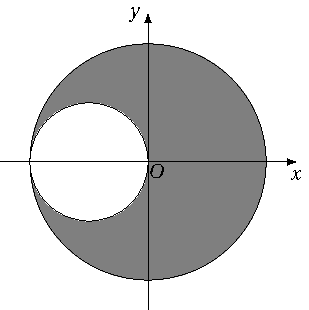
\includegraphics[scale=1]{figure/fig1-5-1.pdf}
			\caption{}\label{fig:1.5.1}
		\end{figure}
	\end{ti}

	\begin{ti}
		设 $D = \bigl\{ (x,y) \bigl| x^{2} + y^{2} \leq 1 \text{\ 且\ } x + y \geq 0 \bigr\}$,$f$ 为连续函数,计算
		\[
			I = \iint_{D} xy \bigl[ x + f\bigl( x^{2} - y^{2} \bigr) \bigr] \dd{x} \dd{y}.
		\]
	\end{ti}

	\begin{ti}
		设 $I(a) = \iint_{D} (x + y) \dd{x} \dd{y}$,其中 $D$ 由直线 $x = a$,$x = 0$,$y = a$,$y = -a$ 及曲线 $x^{2} + y^{2} = ax(a > 0)$ 所围成,计算 $I(a)$.
	\end{ti}

	\begin{ti}
		$\int_{-1}^{1} \dd{x} \int_{|x|}^{\sqrt{2 - x^{2}}} \sin \bigl( x^{2} + y^{2} \bigr) \dd{y} = $\kuo.

		\twoch{$\frac{\uppi}{4}(\cos 2 - 1)$}{$\frac{\uppi}{4}(- \cos 2 + 1)$}{$\frac{\uppi}{4}(\cos 2 + 1)$}{$\frac{\uppi}{4}(- \cos 2 - 1)$}
	\end{ti}

	\begin{ti}
		设平面区域 $D$ 由曲线 $y = \sin x \bigl( - \frac{\uppi}{2} \leq x \leq \frac{\uppi}{2} \bigr)$,$x = -\frac{\uppi}{2}$,$y = 1$ 围成,则 $\iint_{D} \bigl( xy^{3} - 1 \bigr) \dd{\sigma}$ 等于\kuo.

		\fourch{$2$}{$-2$}{$\uppi$}{$-\uppi$}
	\end{ti}

	\begin{ti}
		记平面区域 $D = \bigl\{ (x,y) \bigl| |x| + |y| \leq 1 \bigr\}$,计算如下二重积分:
		\begin{enumerate}
			\item $I_{1} = \iint_{D} \frac{af(x) + bf(y)}{f(x) + f(y)} \dd{\sigma}$,其中 $f(t)$ 为定义在 $(-\infty,$ $+\infty)$ 内的连续正值函数,常数 $a > 0, b > 0$;
			\item $I_{2} = \iint_{D} \bigl( \ee^{\lambda x} - \ee^{-\lambda y} \bigr) \dd{\sigma}$,常数 $\lambda > 0$.
		\end{enumerate}
	\end{ti}

	\begin{ti}
		设 $p(x)$ 在 $[a,b]$ 上非负且连续,$f(x)$ 与 $g(x)$ 在 $[a,b]$ 上连续且有相同的单调性,其中
		\[
			D = \bigl\{ (x,y) \bigl| a \leq x \leq b, a \leq y \leq b \bigr\},
		\]
		比较
		\begin{align*}
			I_{1} &= \iint_{D} p(x) f(x) p(y) g(y) \dd{x} \dd{y},\\
			I_{2} &= \iint_{D} p(x) f(y) p(y) g(y) \dd{x} \dd{y}
		\end{align*}
		的大小,并说明理由.
	\end{ti}
	\subsection{积分比大小}

	\begin{ti}
		设
		\begin{align*}
			a &= \iint_{D} \cos \sqrt{x^{2} + y^{2}} \dd{\sigma},\\
			b &= \iint_{D} \cos \bigl( x^{2} + y^{2} \bigr) \dd{\sigma},\\
			c &= \iint_{D} \cos \bigl( x^{2} + y^{2} \bigr)^{2} \dd{\sigma},
		\end{align*}
		其中 $D = \bigl\{ (x,y) \bigl| x^{2} + y^{2} \leq 1 \bigr\}$,则\kuo.

		\twoch{$c > b > a$}{$a > b > c$}{$b > a > c$}{$c > a > b$}
	\end{ti}

	\begin{ti}
		设平面区域 $D$ 由 $x = 0$,$y = 0$,$x + y = \frac{1}{4}$,$x + y = 1$ 围成,若 $I_{1} = \iint_{D} \bigl[ \ln (x+y) \bigr]^{3} \dd{x} \dd{y}$,$I = \iint_{D} (x + y)^{3} \dd{x} \dd{y}$,$I_{3} = \iint_{D} \bigl[ \sin(x + y) \bigr]^{3} \dd{x} \dd{y}$,则 $I_{1},I_{2},I_{3}$ 的大小顺序为\kuo.

		\twoch{$I_{1} < I_{2} < I_{3}$}{$I_{3} < I_{2} < I_{1}$}{$I_{1} < I_{3} < I_{2}$}{$I_{3} < I_{1} < I_{2}$}
	\end{ti}

	\begin{ti}
		设平面区域 $D = \bigl\{ (x,y) \bigl| (x - 2)^{2} + (y - 1)^{2} \leq 1 \bigr\}$,若比较 $I_{1} = \iint_{D} (x + y)^{2} \dd{\sigma}$ 与 $I_{2} = \iint_{D} (x + y)^{3} \dd{\sigma}$ 的大小,则有\kuo.

		\twoch{$I_{1} = I_{2}$}{$I_{1} > I_{2}$}{$I_{1} < I_{2}$}{不能比较}
	\end{ti}
	\subsection{计算}
	
	\begin{ti}
		计算 $I = \int_{1}^{2} \dd{x} \int_{\frac{1}{x}}^{1} y \ee^{xy} \dd{y}$.
	\end{ti}

	\begin{ti}
		\[
			\int_{0}^{1} \dd{y} \int_{0}^{1} \sqrt{\ee^{2x} - y^{2}} \dd{x} + \int_{1}^{\ee} \dd{y} \int_{\ln y}^{1} \sqrt{\ee^{2x} - y^{2}} \dd{x} = 
		\]
		\kuo.

		\twoch{$\frac{\uppi}{8}\bigl( \ee^{2} - 1 \bigr)$}{$\frac{\uppi}{8}\bigl( \ee^{2} + 1 \bigr)$}{$\frac{\uppi}{4}\bigl( \ee^{2} - 1 \bigr)$}{$\frac{\uppi}{4}\bigl( \ee^{2} + 1 \bigr)$}
	\end{ti}

	\begin{ti}
		已知
		\[
			I = \int_{0}^{2} \dd{x} \int_{0}^{\frac{x^{2}}{2}} f(x,y) \dd{y} + \int_{2}^{2\sqrt{2}} \dd{x} \int_{0}^{\sqrt{8 - x^{2}}} f(x,y) \dd{y},
		\]
		则 $I = $\kuo.

		\onech{$\int_{0}^{2} \dd{y} \int_{\sqrt{2y}}^{\sqrt{8 - y^{2}}} f(x,y) \dd{x}$}{$\int_{0}^{2} \dd{y} \int_{1}^{\sqrt{8 - y^{2}}} f(x,y) \dd{x}$}{$\int_{0}^{1} \dd{y} \int_{\sqrt{2y}}^{\sqrt{8 - y^{2}}} f(x,y) \dd{x}$}{$\int_{0}^{2} \dd{y} \int_{\sqrt{2y}}^{1} f(x,y) \dd{x}$}
	\end{ti}

	\begin{ti}
		累次积分 $\int_{0}^{2R} \dd{y} \int_{0}^{\sqrt{2Ry - y^{2}}} f \bigl( x^{2} + y^{2} \bigr) \dd{x} (R > 0)$ 化为极坐标形式的累次积分为\kuo.

		\onech{$\int_{0}^{\uppi} \dd{\theta} \int_{0}^{2R\sin\theta} f \bigl( r^{2} \bigr) r \dd{r}$}{$\int_{0}^{\frac{\uppi}{2}} \dd{\theta} \int_{0}^{2R\cos\theta} f \bigl( r^{2} \bigr) r \dd{r}$}{$\int_{0}^{\frac{\uppi}{2}} \dd{\theta} \int_{0}^{2R\sin\theta} f \bigl( r^{2} \bigr) r \dd{r}$}{$\int_{0}^{\uppi} \dd{\theta} \int_{0}^{2R\cos\theta} f \bigl( r^{2} \bigr) r \dd{r}$}
	\end{ti}

	\begin{ti}
		计算 $\int_{0}^{1} \dd{y} \int_{\arcsin y}^{\frac{\uppi}{2}} \cos x \cdot \sqrt{1 + \cos^{2}x} \dd{x}$.
	\end{ti}

	\begin{ti}
		计算 $\int_{0}^{1} \dd{y} \int_{3y}^{3} \ee^{x^{2}} \dd{x}$.
	\end{ti}

	\begin{ti}
		计算 $\int_{0}^{1} \dd{y} \int_{\sqrt{y}}^{1} \sqrt{x^{3} + 1} \dd{x}$.
	\end{ti}

	\begin{ti}
		计算 $\int_{0}^{1} \dd{x} \int_{x^{2}}^{1} x^{3} \sin y^{3} \dd{y}$.
	\end{ti}

	\begin{ti}
		计算 $\int_{0}^{1} \dd{x} \int_{x^{2}}^{x} \bigl( x^{2} + y^{2} \bigr)^{-\frac{1}{2}} \dd{y}$.
	\end{ti}

	\begin{ti}
		计算 $\int_{1}^{2} \dd{x} \int_{0}^{x} \frac{y \sqrt{x^{2} + y^{2}}}{x} \dd{y}$.
	\end{ti}

	\begin{ti}
		计算 $\int_{1}^{2} \dd{x} \int_{\sqrt{x}}^{x} \sin \frac{\uppi x}{2y} \dd{y} + \int_{2}^{4} \dd{x} \int_{\sqrt{x}}^{2} \sin \frac{\uppi x}{2y} \dd{y}$.
	\end{ti}

	\begin{ti}
		$\int_{0}^{1} \dd{y} \int_{y}^{1} \Bigl( \frac{\ee^{x^{2}}}{x} - \ee^{y^{2}} \Bigr) \dd{x} = $\htwo.
	\end{ti}

	\begin{ti}
		计算 $\iint_{D} \ee^{\frac{y}{x + y}} \dd{\sigma}$,其中 $D = \bigl\{ (x,y) \bigl| 0 \leq y \leq 1 - x, y \leq x \bigr\}$.
	\end{ti}

	\begin{ti}
		设平面区域 $D = \Bigl\{ (x,y) \Bigl| x^{2} + y^{2} \leq 8, y \geq \frac{x^{2}}{2} \Bigr\}$,计算
		\[
			I = \iint_{D} \bigl[ (x - 1)^{2} + y^{2} \bigr] \dd{\sigma}.
		\]
	\end{ti}

	\begin{ti}
		计算
		\[
			I = \iint_{D} \bigl( x^{2} + xy \bigr)^{2} \dd{x} \dd{y},
		\]
		其中 $D = \bigl\{ (x,y) \bigl| x^{2} + y^{2} \leq 2x \bigr\}$.
	\end{ti}

	\begin{ti}
		计算 $I = \iint_{\sqrt{x} + \sqrt{y} \leq 1} \sqrt[3]{\sqrt{x} + \sqrt{y}} \dd{x} \dd{y}$.
	\end{ti}

	\begin{ti}
		设函数 $f(x,y)$ 连续,且
		\[
			f(x,y) = x + \iint_{D} y f(u,v) \dd{u} \dd{v},
		\]
		其中 $D$ 由 $y = \frac{1}{x}$,$x = 1$,$y = 2$ 围成,求 $f(x,y)$.
	\end{ti}

	\begin{ti}
		设 $D = \bigl\{ (x,y) \bigl| |x| \leq 2, |y| \leq 2 \bigr\}$,计算
		\[
			I = \iint_{D} \bigl| x^{2} + y^{2} - 1 \bigr| \dd{\sigma}.
		\]
	\end{ti}

	\begin{ti}
		设 $D = \bigl\{ (x,y) \bigl| 0 \leq x \leq 1, 0 \leq y \leq 2\ee \bigr\}$,计算
		\[
			\iint_{D} x \bigl| y - \ee^{x} \bigr| \dd{\sigma}.
		\]
	\end{ti}

	\begin{ti}
		计算 $I = \iint_{D} \bigl( |x| + |y| \bigr) \dd{x} \dd{y}$,其中 $D$ 是由曲线 $xy = 2$,直线 $y = x - 1$ 及 $y = x + 1$ 所围成的区域.
	\end{ti}

	\begin{ti}
		设 $D = \bigl\{ (x,y) \bigl| 0 \leq x \leq \uppi, 0 \leq y \leq 2 \bigr\}$,计算 $\iint_{D} \bigl| y - \sin x \bigr| \dd{\sigma}$.
	\end{ti}

	\begin{ti}
		计算
		\[
			I = \int_{-1}^{1} \dd{x} \int_{x}^{2 - |x|} \bigl[ \ee^{|y|} + \sin \bigl( x^{3}y^{3} \bigr) \bigr] \dd{y}.
		\]
	\end{ti}

	\begin{ti}
		设 $f(x,y) = \begin{cases}
			1 - x - y, & x + y \leq 1,\\
			2, & x + y > 1,
		\end{cases}$ 计算
		\[
			\iint_{D} f(x,y) \dd{x} \dd{y},
		\]
		其中 $D$ 为正方形区域 $\bigl\{ (x,y) \bigl| 0 \leq x \leq 1, 0 \leq y \leq 1 \bigr\}$.
	\end{ti}

	\begin{ti}
		设函数 $f(x) = \begin{cases}
			x, & 0 \leq x \leq 2,\\
			0, & x < 0 \text{\ 或\ } x > 2,
		\end{cases}$ 计算 $I = \iint_{D} \frac{f(x + y)}{f\left( \sqrt{x^{2} + y^{2}} \right)} \dd{x} \dd{y}$,其中 $D = \bigl\{ (x,y) \bigl| x^{2} + y^{2} \leq 4 \bigr\}$.
	\end{ti}

	\begin{ti}
		计算 $\iint_{D} \min\bigl\{ x,y \bigr\} \dd{x} \dd{y}$,其中 $D = \bigl\{ (x,y) \bigl| 0 \leq x \leq 3, 0 \leq y \leq 1 \bigr\}$.
	\end{ti}

	\begin{ti}
		计算 $\int_{0}^{a} \dd{x} \int_{0}^{b} \ee^{ \max\left\{ b^{2}x^{2}, a^{2}y^{2} \right\} } \dd{y}$,其中 $a,b > 0$.
	\end{ti}

	\begin{ti}
		设 $F(x,y) = \frac{\partial^{2}f(x,y)}{\partial x \partial y}$ 在 $D = [a,b] \times [c,d]$ 上连续,求
		\[
			I = \iint_{D} F(x,y) \dd{x} \dd{y},
		\]
		并证明:$I \leq 2(M - m)$,其中 $M$ 和 $m$ 分别是 $f(x,y)$ 在 $D$ 上的最大值和最小值.
	\end{ti}

	\begin{ti}
		设函数 $f(x)$ 在 $[0,1]$ 上连续,证明:
		\[
			\int_{0}^{1} \ee^{f(x)} \dd{x} \int_{0}^{1} \ee^{-f(y)} \dd{y} \geq 1.
		\]
	\end{ti}

	\begin{ti}
		设 $f(x,y)$ 为连续函数,则
		\[
			I = \lim_{t \to 0^{+}} \frac{1}{\uppi t^{2}} \iint_{D} f(x,y) \dd{\sigma}
		\] = \htwo,其中 $D = \bigl\{ (x,y) \bigl| x^{2} + y^{2} \leq t^{2} \bigr\}$.
	\end{ti}

	\begin{ti}
		已知 $f(t) = \iint_{D(t): x^{2} + y^{2} \leq t^{2}} \bigl( \ee^{x^{2} + y^{2}} - ky^{2} \bigr) \dd{\sigma}$ 在 $t \in (0,+\infty)$ 内是单调增加函数,$k$为常数,求 $k$ 的最大取值范围.
	\end{ti}

	\begin{ti}
		由曲线 $y = x^{2}$,$y = x + 2$ 所围成的平面薄片,其上各点处的面密度 $\mu = 1 + x^{2}$,则此薄片的质量 $M = $\htwo.
	\end{ti}

	\begin{ti}
		求柱体 $x^{2} + y^{2} \leq 2x$ 被 $x^{2} + y^{2} + z^{2} = 4$ 所截得部分的体积.
	\end{ti}

	\begin{ti}
		设平面薄片所占的区域 $D$ 由抛物线 $y = x^{2}$ 及直线 $y = x$ 所围成,它在 $(x,y)$ 处的面密度 $\rho(x,y) = x^{2}y$,求此薄片的重心.
	\end{ti}